\chapter{贝叶斯优化}
\label{chap:bayesian-optimization}

一次流体仿真要跑四个小时，它有一个需要调节的参数，我们希望输出误差尽量小。仿真程序是一个不透明的黑箱，给它一个参数，它还回一个数，不给导数。这周的算力只够运行六次。第六次运行结束时必须交出一个参数值，往后就按它使用。六次机会应该怎么花？

第~\ref{chap:zeroth-order-optimization}章用函数值差分构造局部方向，第~\ref{chap:random-search}章靠大量候选的提议和淘汰探索解空间，这两条路都假定评价次数可以比较多。评价极贵时，每一次评价之后都值得停下来，把已有读数全部用上，认真想一想下一次该放在哪里。\term{贝叶斯优化}（Bayesian optimization）就是把这件事组织成计算的办法：用已完成的读数建立一个带不确定性的概率模型，再按潜在收益和不确定性决定下一次评价。

全章用一个一维仿真例子贯穿。我们先说清问题里“评价点”和“最终推荐”的区别，再建立高斯过程这个概率模型，然后比较几种把模型变成选点分数的规则，把它们接成一个完整的循环。之后依次放宽理想假设，讨论读数有噪声、约束也要试验才知道、多个试验同时运行三种情形。最后回答预算怎样核算，最终结果怎样评价，以及哪些结论有理论保证、在什么条件下成立。

\section{昂贵黑箱问题}
\label{sec:bo-problem}

只有$T$次昂贵评价时，优化问题应当怎样提？设搜索域$\bm{C}\subseteq\mathbb{R}^n$已知，目标$f:\bm{C}\to\mathbb{R}$的表达式未知，要解的是
\begin{equation}
 \min_{\bm{x}\in\bm{C}}\ f(\bm{x}),
 \label{eq:bo-problem}
\end{equation}
其中每次只能选一个$\bm{x}$，付出一次运行的代价，读到一个函数值。这类只能通过读数了解目标的问题称为\term{黑箱优化}（black-box optimization）。

与前面各章不同，这里最先固定的不是精度，而是预算：允许多少次评价，或者总共多少运行时间。问题随之变成“这$T$次机会怎样分配”。机会要分给两类地方：看起来有希望的区域，以及几乎一无所知的区域。只去前者可能错过别处更深的谷，只去后者又用不上已经学到的东西。

\paragraph{贯穿全章的例子}
设仿真参数$x$在$\bm{C}=[0,8]$内取值，输出误差$f(x)$已作标准化，负值表示比基准好，预算$T=6$。表~\ref{tab:bo-readings}列出整数位置上的读数。真实计算时这张表并不存在，算法只会知道被评价过的那几列；把它写出来是为了让后面的每一步都可以核对。

\begin{BookInlineTable}
 \centering
 \caption{贯穿例的整数位置读数。函数$f$是过这九个点的自然三次样条，只作为教学假设，算法不知道它。}
 \label{tab:bo-readings}
 \begin{tabular}{cccccccccc}
 \toprule
 $x$&0&1&2&3&4&5&6&7&8\\
 \midrule
 $f(x)$&0.9&0.2&$-0.5$&0.1&0.7&0.3&$-1.0$&$-0.3$&0.8\\
 \bottomrule
 \end{tabular}
\end{BookInlineTable}

这个函数有两个谷，一个在$x=2$附近，另一个在$x=6$附近，后者更深。样条的最小值约为$-1.029$，在$x\approx6.13$处取得。

\subsection{评价点与推荐解}
\label{sec:bo-query-recommend}

六次评价结束后要交出一个答案。答案未必是读数最好的那次，也未必是评价过的点。为了不把两件事混在一起，需要分开两个角色：\emph{评价点}用来收集信息，\emph{推荐解}用来实际采用。

图~\ref{fig:bo-query-recommend}是后面算法在贯穿例上实际走出的六次评价，数字是评价的先后。第$4$次去了$x=8$，读数$0.8$很差，从目标值看是一次失败。可是它告诉我们右端不值得再投入，这对后面的判断有用。第$5$次在$x=6$读到$-1.0$，于是最终推荐$\widehat{x}_6=6$。第$6$次在$x=0$的读数$0.9$又差得多，但这并不影响推荐，因为推荐解不需要是最后一次评价。

\begin{BookInlineFigure}
 \centering
 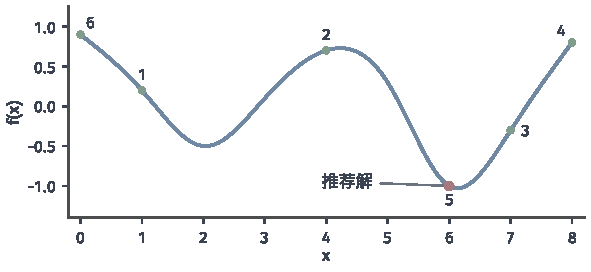
\includegraphics[width=100mm]{figures/05-optimization/05-stochastic-optimization/matplotlib/bo-query-recommend/figure.pdf}
 \caption{评价点与推荐解。蓝线是目标$f$，绿点是六次评价，旁边的数字是评价顺序，红点是最终推荐。第$4$次和第$6$次的读数很差，它们的任务是收集信息，不是交付答案。}
 \label{fig:bo-query-recommend}
\end{BookInlineFigure}

用数据集合记录当前已有的信息。设前$t$次评价的位置与读数为$(\bm{x}_i,y_i)$，记
\begin{equation}
 \mathcal{D}_t=\{(\bm{x}_i,y_i)\}_{i=1}^t.
 \label{eq:bo-data}
\end{equation}
这里下标$i$表示第$i$次评价，因为后面总要同时引用多次评价的位置，所以本章把评价序号写在下标。

选点规则必须遵守时间次序：第$t+1$个评价点只能依赖$\mathcal{D}_t$，至多再加上与目标无关的随机数，不能用尚未返回的读数。图~\ref{fig:bo-info-timeline}画出了这个次序。这条要求看似多余，实际很有约束力。比较不同方法时，若某个方法的超参数是用全部读数调好的，它在前几步就已用到了未来的信息，比较便不公平。

\begin{BookInlineFigure}
 \centering
 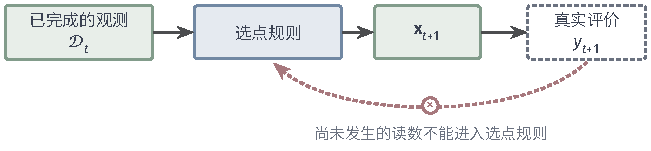
\includegraphics[width=110mm]{figures/05-optimization/05-stochastic-optimization/tikz/bo-info-timeline/figure.pdf}
 \caption{选点规则可以使用的信息。选点规则只读取已完成的观测$\mathcal{D}_t$，下一次评价的读数$y_{t+1}$在选点之后才产生（虚线框），红色虚线表示这条信息通路不允许存在。}
 \label{fig:bo-info-timeline}
\end{BookInlineFigure}

\subsection{概率模型的作用}
\label{sec:bo-probability-role}

只有三个读数时，$x=6$处的函数值是多少？我们不知道，但并非毫无看法：离读数近的地方函数值大概与读数接近，离得远的地方拿不准。要把“大概”和“拿不准”写成可以计算的东西，需要给未知的$f$配一个概率描述。

这里最容易误解的一点是，$f$本身并不随机。仿真程序是确定的，同一个$x$每次算出同样的结果，只是我们不知道结果。概率描述的是我们的认识状态，不是目标的物理性质。做法是引入一个随机函数$F$作为模型，把$f$看成它可能的一种情形。在看到数据之前，$F$的分布称为\term{先验}（prior）；把$\mathcal{D}_t$作为条件之后，$F$的分布称为\term{后验}（posterior）。

后验分布的变化，表示认识变了，不表示目标变了。可以把它想成一张还在绘制中的地形图：实地地形一直没动，测过的点清晰，没测过的地方模糊，每多测一点，图就清楚一些。这个比方有一处不准确：地形图的模糊只来自没测量，而概率模型的结论还依赖我们事先对地形光滑程度的假设，假设错了，图可能清晰却画错了。

图~\ref{fig:bo-consistent-functions}中的紫线是在$x=1,4,7$三个读数条件下，从模型里抽取的几条函数。它们都穿过三个读数，在读数之间各走各的路。蓝线是真实目标，只有一条，它在整个过程中不改变。浅蓝带是模型认为函数值大致所在的范围，读数处收成一点，远离读数时变宽。下一次评价的放置，就要根据这种“哪里可能低、哪里还拿不准”的信息来定。

\begin{BookInlineFigure}
 \centering
 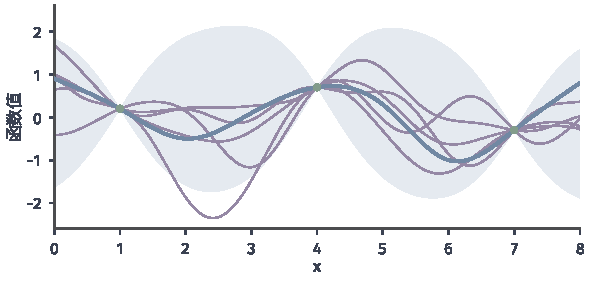
\includegraphics[width=100mm]{figures/05-optimization/05-stochastic-optimization/matplotlib/bo-consistent-functions/figure.pdf}
 \caption{固定的目标与模型的多种可能。粗蓝线是真实目标$f$，绿点是$x=1,4,7$的读数，细紫线是后验分布的五个样本，浅蓝带是后验均值上下各两倍标准差。五条紫线都与读数相符，它们的差异表示认识的不确定，不表示$f$在变化。}
 \label{fig:bo-consistent-functions}
\end{BookInlineFigure}

概率模型是本章区别于前两章的关键。三章都可以只用函数值，分工却在于用这些值做什么，表~\ref{tab:bo-three-methods}作了对比。也要注意，“贝叶斯”这个词不意味着算法每步都在抽签。后面的期望改进给定$\mathcal{D}_t$后完全确定，只有Thompson采样这样的规则才主动使用随机数。

\begin{BookInlineTable}
 \centering
 \caption{三种只用函数值的做法。}
 \label{tab:bo-three-methods}
 \begin{tabular}{lll}
 \toprule
 &用读数做什么&适合的评价预算\\
 \midrule
 零阶随机优化&差分成局部方向&较多，随维数增长\\
 随机搜索&更新搜索状态或分布&较多，候选大量淘汰\\
 贝叶斯优化&建模后计算下次评价的价值&很少，每次都很贵\\
 \bottomrule
 \end{tabular}
\end{BookInlineTable}

\section{概率代理}
\label{sec:bo-surrogate}

怎样用一个读数更新没有被评价的位置的认识？这要求模型做到两件事，一是对每个候选点给出可能函数值的分布，二是说清不同位置之间怎样关联，否则一个位置的读数对其他位置不起作用。满足这两点、用来代替昂贵目标接受查询的模型，称为\term{概率代理}（probabilistic surrogate）。

本节以高斯过程为主说明这个接口。贝叶斯优化并不依赖高斯过程，只要模型能给出相应的预测分布，例如贝叶斯神经网络、树模型的集成，也可以代入后面的选点规则，只是计算的具体公式不同。

\subsection{高斯过程先验}
\label{sec:bo-gp-prior}

先看模型要表达的直觉：相近的参数，通常给出相近的仿真结果。这句话有两层意思。其一，单看一个位置，函数值可能的范围是一个分布。其二，两个位置离得越近，它们的函数值越同涨同落。用协方差描述第二层意思最直接，而最便于计算的联合分布是多元高斯分布。

\begin{definition}[高斯过程]
\label{def:bo-gp}
设$m_0:\bm{C}\to\mathbb{R}$，$k:\bm{C}\times\bm{C}\to\mathbb{R}$。若对任意有限个点$\bm{x}_1,\ldots,\bm{x}_n\in\bm{C}$，向量$(F(\bm{x}_1),\ldots,F(\bm{x}_n))^\top$都服从多元高斯分布，且
\begin{equation}
 \mathbb{E}[F(\bm{x})]=m_0(\bm{x}),\qquad
 \operatorname{Cov}(F(\bm{x}),F(\bm{x}'))=k(\bm{x},\bm{x}'),
 \label{eq:bo-gp}
\end{equation}
就称随机函数$F$是以$m_0$为\term{均值函数}（mean function）、以$k$为\term{协方差核}（covariance kernel）的\term{高斯过程}（Gaussian process，GP）。
\end{definition}

定义只谈有限个点，这正是它好用的地方。一次计算只会碰到有限个位置，手头需要的总是一个普通的多元高斯分布。

核$k$不能随便写。把几个位置的函数值作线性组合，方差必须非负。对任意实数$a_1,\ldots,a_n$，
\[
 0\leq\operatorname{Var}\Bigl(\sum_{i=1}^n a_iF(\bm{x}_i)\Bigr)
 =\sum_{i=1}^n\sum_{j=1}^n a_ia_jk(\bm{x}_i,\bm{x}_j)
 =\bm{a}^\top\bm{K}\bm{a},
\]
其中$\bm{K}$是元素为$k(\bm{x}_i,\bm{x}_j)$的矩阵。所以$k$必须对称，且任意有限组点上的$\bm{K}$都半正定。反过来，满足这两条的$k$配上任意均值函数，确实对应一个高斯过程，证明要用到有限维分布族的相容性与延拓定理，这里只使用结论。

\paragraph{贯穿例的核}
本章取$m_0\equiv0$，并取
\begin{equation}
 k(x,x')=2^{-(x-x')^2}.
 \label{eq:bo-example-kernel}
\end{equation}
它是常用的\term{平方指数核}（squared exponential kernel）$\exp(-(x-x')^2/(2\ell^2))$在$\ell^2=1/(2\ln2)$时的情形，$\ell\approx0.85$。选这个数只是为了手算：间距$1,2,3$的相关系数分别是$1/2,1/16,1/512$。先验方差$k(x,x)=1$表示模型认为函数值大致在$\pm2$内，这与表~\ref{tab:bo-readings}的数量级相符。

取三个相邻位置$x=3,4,5$，核矩阵为
\[
 \bm{K}=\begin{bmatrix}1&1/2&1/16\\1/2&1&1/2\\1/16&1/2&1\end{bmatrix}.
\]
三个顺序主子式依次为
\[
 1,\qquad \frac34,\qquad \frac{135}{256},
\]
全部为正，所以这个$\bm{K}$正定。

\paragraph{核规定了模型愿意相信的变化尺度}
参数$\ell$称为\term{长度尺度}（length scale），它回答“隔多远的两个点就基本无关了”。图~\ref{fig:bo-kernel-scales}比较了三个取值。$\ell$小时相关性衰减快，先验样本频繁起伏；$\ell$大时样本缓慢变化。三条样本用的是同一组随机数，差别完全来自核。

\begin{BookInlineFigure}
 \centering
 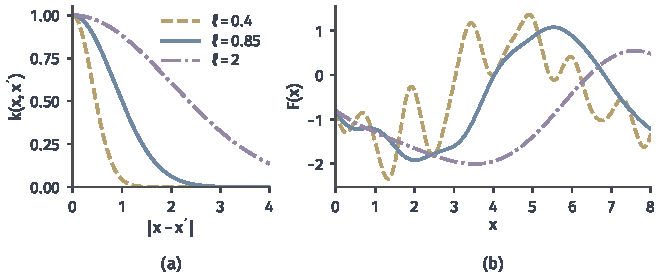
\includegraphics[width=112mm]{figures/05-optimization/05-stochastic-optimization/matplotlib/bo-kernel-scales/figure.pdf}
 \caption{长度尺度的作用。(a)平方指数核随距离的衰减，$\ell=0.85$是贯穿例的取值。(b)用同一组标准正态随机数生成的三条先验样本，线型与(a)对应。长度尺度越大，样本越缓慢。}
 \label{fig:bo-kernel-scales}
\end{BookInlineFigure}

所以核不只是计算工具，它是我们事先下的一个赌注。选了$\ell$，就等于声明目标不会比这个尺度变化得更快。这一声明可能错，第~\ref{sec:bo-model-specification}节专门讨论错了会怎样。

\subsection{后验预测}
\label{sec:bo-posterior}

先用两个位置看清更新是怎么发生的。考虑$x=3$和$x=4$，由式~\eqref{eq:bo-example-kernel}，
\[
 \begin{bmatrix}F(3)\\F(4)\end{bmatrix}
 \sim N\left(\begin{bmatrix}0\\0\end{bmatrix},
 \begin{bmatrix}1&1/2\\1/2&1\end{bmatrix}\right).
\]
现在只评价$x=3$，无噪声地读到$F(3)=1$。关键是把$F(4)$拆成“能由$F(3)$解释的部分”和“剩余部分”：
\[
 F(4)=\tfrac12F(3)+R.
\]

系数$1/2$的选法是让$R$与$F(3)$不相关：
\[
 \operatorname{Cov}(R,F(3))=\tfrac12-\tfrac12\cdot1=0.
\]
联合高斯时不相关就意味着独立，所以读到$F(3)$不改变$R$的分布。$R$的方差为
\[
 \operatorname{Var}(R)=1-2\cdot\tfrac12\cdot\tfrac12+\tfrac14\cdot1=\tfrac34.
\]
代入$F(3)=1$，得到
\[
 F(4)\mid F(3)=1\ \sim\ N\bigl(\tfrac12,\tfrac34\bigr).
\]

虽然没有评价$x=4$，这里的均值从$0$变成了$0.5$，方差从$1$降到了$0.75$。图~\ref{fig:bo-conditional-slice}中，(a)的椭圆是联合分布的等高线，在$F(3)=1$处竖切一刀，得到(b)中的绿线。椭圆是斜的，切线才偏离中心；若相关系数为$0$，椭圆不倾斜，切出来的分布就和先验一样，读数不传递任何信息。

\begin{BookInlineFigure}
 \centering
 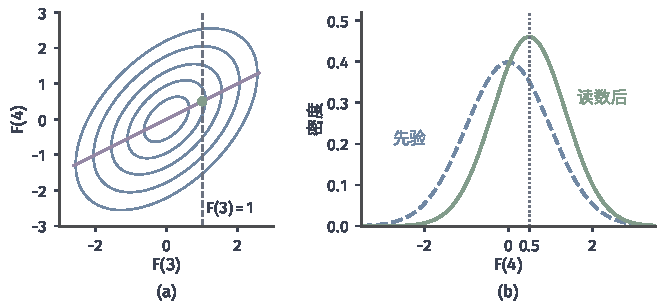
\includegraphics[width=112mm]{figures/05-optimization/05-stochastic-optimization/matplotlib/bo-conditional-slice/figure.pdf}
 \caption{读数怎样传到相关的位置。(a)蓝色椭圆是$(F(3),F(4))$的联合分布等高线，相关系数$1/2$，紫线是条件均值$F(4)=F(3)/2$，竖虚线是读数$F(3)=1$，绿点是该读数下$F(4)$的条件均值。(b)蓝虚线是$F(4)$的先验$N(0,1)$，绿线是读数后的$N(1/2,3/4)$。}
 \label{fig:bo-conditional-slice}
\end{BookInlineFigure}

一般情形只是把这种拆分写成矩阵。记$\bm{K}_t$为$t\times t$矩阵，元素是$k(\bm{x}_i,\bm{x}_j)$；$\bm{k}_t(\bm{x})$是长度$t$的向量，第$i$个分量是$k(\bm{x},\bm{x}_i)$；$\bm{y}_t$是读数向量；$\bm{m}_{0,t}$是先验均值在各评价点处的取值。读数可能含噪，设$y_i=F(\bm{x}_i)+\varepsilon_i$，$\varepsilon_i\sim N(0,\tau^2)$，彼此独立，且与$F$独立；$\tau=0$表示无噪声。

\begin{theorem}[高斯过程的后验]
\label{thm:bo-posterior}
设$F$是高斯过程，评价点固定，核与噪声参数已知，$\bm{A}_t=\bm{K}_t+\tau^2\bm{I}$可逆。则给定$\bm{y}_t$，$F$仍是高斯过程，其后验均值与后验协方差为
\begin{align}
 m_t(\bm{x})&=m_0(\bm{x})+\bm{k}_t(\bm{x})^\top\bm{A}_t^{-1}(\bm{y}_t-\bm{m}_{0,t}),
 \label{eq:bo-post-mean}\\
 c_t(\bm{x},\bm{x}')&=k(\bm{x},\bm{x}')-\bm{k}_t(\bm{x})^\top\bm{A}_t^{-1}\bm{k}_t(\bm{x}').
 \label{eq:bo-post-cov}
\end{align}
特别地，记$s_t^2(\bm{x})=c_t(\bm{x},\bm{x})$，则
\begin{equation}
 F(\bm{x})\mid\mathcal{D}_t\sim N\bigl(m_t(\bm{x}),s_t^2(\bm{x})\bigr).
 \label{eq:bo-post-marginal}
\end{equation}
\end{theorem}

\begin{proof}
取任意有限组候选点，$F$在这些点与读数向量合起来是联合高斯的。对一个候选点$\bm{x}$，令
\[
 \bm{a}=\bm{A}_t^{-1}\bm{k}_t(\bm{x}).
\]
定义剩余量
\[
 R(\bm{x})=F(\bm{x})-m_0(\bm{x})-\bm{a}^\top(\bm{y}_t-\bm{m}_{0,t}),
\]
这里$\bm{y}_t$理解为随机向量。

读数的协方差矩阵是$\bm{A}_t$，$F(\bm{x})$与读数的协方差向量是$\bm{k}_t(\bm{x})$，于是
\[
 \operatorname{Cov}(R(\bm{x}),\bm{y}_t)=\bm{k}_t(\bm{x})-\bm{A}_t\bm{a}=\bm{0}.
\]
联合高斯下，不相关推出独立，所以$\mathcal{D}_t$不改变$R(\bm{x})$的分布，它的均值仍是$0$。把读数的实际值代入$F(\bm{x})$的分解式，条件均值就是式~\eqref{eq:bo-post-mean}。

设$R'$是$\bm{x}'$处对应的剩余量，$\bm{a}'=\bm{A}_t^{-1}\bm{k}_t(\bm{x}')$。给定读数后$F(\bm{x})$与$F(\bm{x}')$的随机部分只有$R$与$R'$，因此
\[
 \begin{aligned}
 \operatorname{Cov}(R,R')
 &=k(\bm{x},\bm{x}')-\bm{a}^\top\bm{k}_t(\bm{x}')-\bm{a}'^\top\bm{k}_t(\bm{x})+\bm{a}^\top\bm{A}_t\bm{a}'\\
 &=k(\bm{x},\bm{x}')-\bm{k}_t(\bm{x})^\top\bm{A}_t^{-1}\bm{k}_t(\bm{x}').
 \end{aligned}
\]
这就是式~\eqref{eq:bo-post-cov}。任意有限组点上同样成立，所以后验仍是高斯过程。
\end{proof}

这个证明用到联合高斯下不相关推出独立，条件高斯的一般公式及其矩阵推导可参考\BookChapterRef{chap:random-vectors}{卷七第6章“随机向量”}；把核视为函数上的先验来做回归的一般理论，可参考\BookChapterRef{chap:nonparametric-inference}{卷八第2章“非参数分布与函数推断”}。

读这两个公式时，注意三件事。第一，后验方差~\eqref{eq:bo-post-cov}不含读数$\bm{y}_t$，只取决于评价放在哪里，好读数和坏读数减少的不确定性相同。第二，无噪声时$m_t(\bm{x}_i)=y_i$，$s_t(\bm{x}_i)=0$，模型穿过读数。第三，$c_t(\bm{x},\bm{x}')$要保留，不能只留方差，后面联合抽样和批量选点都要用到不同候选点之间的后验协方差。

定理假设评价点固定，而实际的$\bm{x}_{t+1}$依赖之前的读数。公式仍然成立，原因是选点规则只看$\mathcal{D}_t$：写出整条数据的似然时，选点这一步给出的因子不依赖$F$，它在归一化时被消去，后验仍只由读数的高斯因子决定。条件分布的一般含义可参考\BookChapterRef{chap:conditional-expectation}{卷七第10章“条件期望”}。

\paragraph{贯穿例：三个读数后的后验}
评价$x=1,4,7$，读数$\bm{y}_3=(0.2,0.7,-0.3)^\top$。核矩阵是
\[
 \bm{K}_3=\begin{bmatrix}1&2^{-9}&2^{-36}\\2^{-9}&1&2^{-9}\\2^{-36}&2^{-9}&1\end{bmatrix},
\]
其中$2^{-9}\approx0.002$。解线性方程$\bm{K}_3\bm{w}=\bm{y}_3$，得到
\[
 \bm{w}=\bm{K}_3^{-1}\bm{y}_3\approx(0.1986,\ 0.7002,\ -0.3014)^\top.
\]

看未评价的$x=6$。到三个评价点的距离是$5,2,1$，所以
\[
 \bm{k}_3(6)=(2^{-25},\ 1/16,\ 1/2)^\top.
\]
由式~\eqref{eq:bo-post-mean}，
\[
 m_3(6)=\bm{k}_3(6)^\top\bm{w}\approx0.0625\times0.7002-0.5\times0.3014\approx-0.107.
\]
由式~\eqref{eq:bo-post-cov}，
\[
 s_3^2(6)=1-\bm{k}_3(6)^\top\bm{K}_3^{-1}\bm{k}_3(6)\approx0.746,
\]
即$s_3(6)\approx0.864$。把$2^{-9}$按$0$手算，会得到$-0.106$和$0.746$，差别只在第三位小数。

图~\ref{fig:bo-posterior-sequence}是读数逐个加入时的后验。第一个读数只影响$x=1$附近，其他地方后验几乎还是先验。后面的读数逐段收紧不确定带。深色的后验均值并没有“找到”$x=6$的谷，这很自然：三个点都不在谷里，模型没有理由想象到它。正是这种“均值还不低、但不确定带向下伸得很远”的区域，需要由下一节的规则来评估。

\begin{BookInlineFigure}
 \centering
 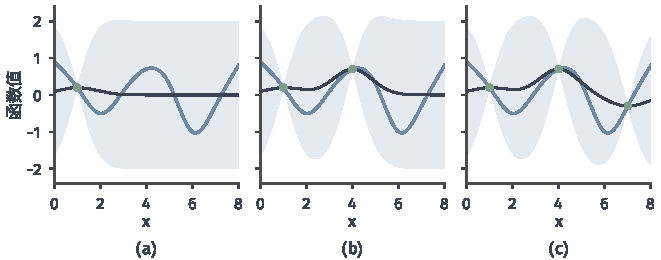
\includegraphics[width=112mm]{figures/05-optimization/05-stochastic-optimization/matplotlib/bo-posterior-sequence/figure.pdf}
 \caption{后验随读数更新。蓝线是目标$f$，深色线是后验均值$m_t$，浅蓝带是$m_t\pm2s_t$，绿点是读数。(a)只有$x=1$；(b)加入$x=4$；(c)加入$x=7$。}
 \label{fig:bo-posterior-sequence}
\end{BookInlineFigure}

计算量也要记一笔。对$\bm{A}_t$作一次Cholesky分解约需$t^3/3$次运算，见\BookChapterRef{chap:direct-linear-solvers}{卷二第12章“线性方程的直接求解”}；此后每个候选点的均值需$O(t)$次运算，方差需$O(t^2)$次。贝叶斯优化中$t$通常只有几十到几百，这笔开销相对一次昂贵评价可以忽略，第~\ref{sec:bo-budget}节再核算它什么时候不能忽略。

\subsection{模型设定}
\label{sec:bo-model-specification}

上面都假定核与噪声参数已知。实际问题中$\ell$、先验方差等\term{超参数}（hyperparameter）并不知道，这就有了本节的问题：模型的这些设定错了会怎样，又该如何对待它们的不确定性。

\paragraph{边缘似然与直接代入}
常用办法是看哪组超参数最能解释已有读数。把超参数记为$\bm{\theta}$，读数的边缘分布是$N(\bm{m}_{0,t},\bm{A}_t(\bm{\theta}))$，其对数密度
\begin{equation}
 \log p(\bm{y}_t\mid\bm{\theta})=-\tfrac12\bm{r}^\top\bm{A}_t^{-1}\bm{r}-\tfrac12\log\det\bm{A}_t-\tfrac t2\log(2\pi)
 \label{eq:bo-marginal-likelihood}
\end{equation}
称为\term{边缘似然}（marginal likelihood）的对数，其中$\bm{r}=\bm{y}_t-\bm{m}_{0,t}$。第一项奖励拟合读数，第二项惩罚过于灵活的模型。常见做法是取使它最大的$\widehat{\bm{\theta}}$，然后把它当作真值代入定理~\ref{thm:bo-posterior}。

直接代入回避了一个事实：超参数本身也拿不准。把不确定性计入的做法是对超参数的后验分布积分，得到混合预测。若$\bm{\theta}$只有有限个候选，后验概率为$w_j$，候选$j$给出的均值和方差为$m^{(j)},v^{(j)}$，则由全方差公式，
\begin{equation}
 \begin{gathered}
 \bar m=\sum_jw_jm^{(j)},\\
 \bar v=\sum_jw_jv^{(j)}+\sum_jw_j\bigl(m^{(j)}-\bar m\bigr)^2.
 \end{gathered}
 \label{eq:bo-mixture}
\end{equation}
第一项是平均的方差，第二项是不同超参数之间的分歧。第二项非负，所以混合预测的方差不小于各候选方差的加权平均，分歧越大增加越多。

\paragraph{例：两个候选长度尺度}
仍用三个读数，比较$\ell\approx0.85$和$\ell=3$，两者的先验概率相等。由式~\eqref{eq:bo-marginal-likelihood}算得对数边缘似然分别约为$-3.067$和$-3.106$，几乎相同，按贝叶斯公式得到后验概率
\[
 w_1\approx0.51,\qquad w_2\approx0.49.
\]
三个读数不足以区分这两种解释。

两种解释在$x=6$处的预测却差得很远：
\[
 \begin{aligned}
 \ell\approx0.85:&\quad m=-0.107,\quad v=0.746,\\
 \ell=3:&\quad m=0.093,\quad v=0.015.
 \end{aligned}
\]
由式~\eqref{eq:bo-mixture}，混合预测的均值和方差为
\[
 \bar m\approx-0.009,\qquad \bar v\approx0.398.
\]

若只取$\ell=3$直接代入，方差$0.015$比混合预测小了约$26$倍。图~\ref{fig:bo-model-specification}(b)显示，长度尺度大的模型在$x=6$处把标准差算得很小，而真实值$-1.0$远在它的不确定带之外。这正是直接代入的风险：边缘似然选中了一个看上去同样好的解释，却丢掉了“还有另一种解释”这条信息。

\begin{BookInlineFigure}
 \centering
 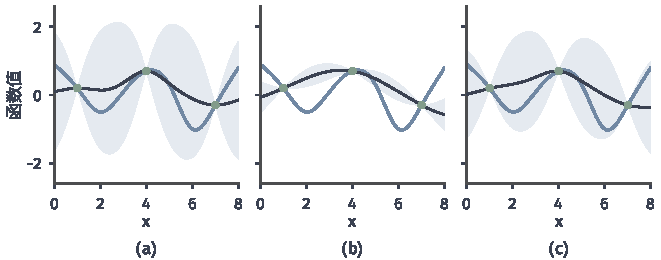
\includegraphics[width=112mm]{figures/05-optimization/05-stochastic-optimization/matplotlib/bo-model-specification/figure.pdf}
 \caption{同样三个读数下的不同模型设定。蓝线是目标，深色线是预测均值，浅蓝带是均值上下两倍标准差。(a)$\ell\approx0.85$；(b)$\ell=3$，不确定带很窄，却没有盖住$x=6$附近的谷；(c)两者按边缘似然加权的混合预测，读数之间的方差反映了两种解释的分歧。}
 \label{fig:bo-model-specification}
\end{BookInlineFigure}

\paragraph{设定要回到问题来检查}
长度尺度隐含一个假设：同样的距离代表同样的变化幅度。输入的尺度是否合适直接关系这个假设。例如学习率类的参数从$10^{-4}$变到$1$，在原始坐标上$10^{-4}$与$10^{-3}$几乎重合，但它们的效果可能相差很多；改用$\log_{10}$坐标后，相邻量级的距离才都等于$1$。多维问题中各坐标的单位不同，通常给每个坐标各设一个长度尺度。

先验的光滑程度也要与问题相符。平方指数核的样本无穷次可微，目标若有折点或跳跃，模型会用过短的长度尺度去迁就，导致全局方差偏大。可微性有限的核，如Mat\'ern族，常用来表达较弱的光滑假设。

读数本身可以检验模型。依次去掉第$i$个读数，用其余读数预测它，得到留一标准化残差
\begin{equation}
 e_i=\frac{y_i-m_{-i}(\bm{x}_i)}{\sqrt{s_{-i}^2(\bm{x}_i)+\tau^2}}.
 \label{eq:bo-loo}
\end{equation}
模型合适时这些数大致像标准正态的取值，大量绝对值超过$3$说明模型与读数不符。贯穿例的三个读数相距较远，其余读数几乎不影响被去掉的位置，$e_i$约等于读数本身，$0.2,0.7,-0.3$都不大。可是读数太少时这个检查的力量也很弱，通过检查不等于模型正确。

低方差只说明“在这个模型下”不确定性小，不能直接等同于目标已经被准确掌握。图~\ref{fig:bo-model-specification}(b)是一个具体的反例。后面几节的后验都默认超参数固定，这是为了把选点逻辑讲清楚；实际使用时，每轮通常重新估计或积分超参数，第~\ref{sec:bo-noise-variances}节还会看到这样做对方差的影响。

\section{采集函数}
\label{sec:bo-acquisition}

后验告诉了我们每个候选点上函数值的分布，但它没有说下一次该评价哪里。接下来要弄清：怎样把后验转成一个可以比较大小的分数？这个分数称为\term{采集函数}（acquisition function），记作$\alpha_t(\bm{x})$，下一个评价点取使它最大的位置。

好的分数要处理一对矛盾。后验均值低的地方看起来有希望，这是\emph{利用}；后验方差大的地方我们知之甚少，那里可能藏着好东西，这是\emph{探索}。各种采集函数的差别就在于用什么方式把两者结合起来。

本节先假定观测无噪声，当前已观测的最好值就是
\begin{equation}
 b_t=\min_{i\leq t}f(\bm{x}_i).
 \label{eq:bo-incumbent}
\end{equation}
下面统一按最小化比较。例子都用$t=3$时贯穿例的后验，$b_3=-0.3$，取整数候选点。

\subsection{改进概率（PI）}
\label{sec:bo-pi}

最朴素的想法是问：在这个位置评价，有多大可能比现在最好的结果更好？再要求至少好出一个幅度$\xi\geq0$，得到\term{改进概率}（probability of improvement，PI）：
\begin{equation}
 \mathrm{PI}_t(\bm{x})=\mathbb{P}\bigl(F(\bm{x})<b_t-\xi\mid\mathcal{D}_t\bigr)
 =\Phi\left(\frac{b_t-\xi-m_t(\bm{x})}{s_t(\bm{x})}\right),
 \label{eq:bo-pi}
\end{equation}
其中$s_t(\bm{x})>0$，$\Phi$是标准正态分布函数。$s_t(\bm{x})=0$时，函数值已确定，$\mathrm{PI}$依$m_t(\bm{x})<b_t-\xi$是否成立取$1$或$0$。

PI只数“是否过线”，不问过线之后好多少。比较两个候选，取$b_t=0$，$\xi=0$，
\[
 \text{A}:\ F\sim N(-0.1,\ 0.1^2),\qquad
 \text{B}:\ F\sim N(0.5,\ 1).
\]
代入式~\eqref{eq:bo-pi}，
\[
 \mathrm{PI}(\text{A})=\Phi(1)\approx0.841,\qquad
 \mathrm{PI}(\text{B})=\Phi(-0.5)\approx0.309.
\]
PI选A。图~\ref{fig:bo-pi-vs-ei}的绿色面积就是这两个概率。可是A即使成功也只改善零点几，B虽不常成功，一旦成功可能改善很多。

\begin{BookInlineFigure}
 \centering
 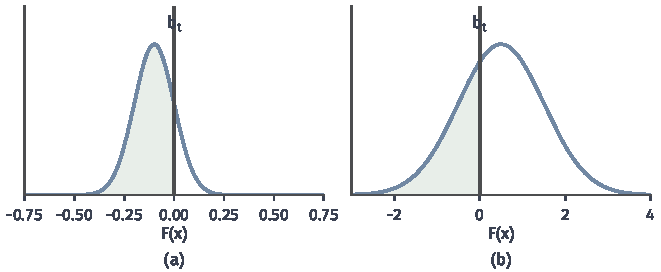
\includegraphics[width=112mm]{figures/05-optimization/05-stochastic-optimization/matplotlib/bo-pi-vs-ei/figure.pdf}
 \caption{改进的概率与幅度。蓝线是候选点函数值的后验密度，深灰竖线是当前最好值$b_t=0$，浅绿面积是改进概率。(a)候选A：$N(-0.1,0.1^2)$，大概率过线，但过线幅度很小。(b)候选B：$N(0.5,1)$，概率较小，但左尾可以伸得很远。两图横轴比例不同。}
 \label{fig:bo-pi-vs-ei}
\end{BookInlineFigure}

$\xi$的作用可以这样看。$\xi=0$时，紧贴着当前最好点的位置，后验均值几乎等于$b_t$，方差几乎为零，PI接近$1/2$，后面的图中可以看到，PI的最大点恰好贴在已观测的最好点旁边，这样的评价几乎不提供新信息。取$\xi>0$把门槛压低，这种贴边的小改进就不算数了。可是$\xi$取多大没有普适答案，它取决于函数值的尺度。

\subsection{期望改进（EI）}
\label{sec:bo-ei}

PI的缺陷指明了修改方向：把幅度也算进去。若在$\bm{x}$评价，新的最好值相比$b_t$的改善量是
\[
 \bigl(b_t-F(\bm{x})\bigr)_+=\max\{b_t-F(\bm{x}),0\}.
\]
没有改善时计为$0$，因为最好值不会变差。这个改善量的后验期望称为\term{期望改进}（expected improvement，EI）：
\begin{equation}
 \mathrm{EI}_t(\bm{x})=\mathbb{E}\bigl[(b_t-F(\bm{x}))_+\mid\mathcal{D}_t\bigr].
 \label{eq:bo-ei-def}
\end{equation}

\begin{theorem}[期望改进的闭式]
\label{thm:bo-ei}
设$F(\bm{x})\mid\mathcal{D}_t\sim N(m,s^2)$。若$s>0$，记$z=(b_t-m)/s$，则
\begin{equation}
 \mathrm{EI}_t(\bm{x})=(b_t-m)\Phi(z)+s\phi(z),
 \label{eq:bo-ei}
\end{equation}
其中$\Phi$、$\phi$分别是标准正态分布函数和密度函数。若$s=0$，则
\begin{equation}
 \mathrm{EI}_t(\bm{x})=(b_t-m)_+.
 \label{eq:bo-ei-zero}
\end{equation}
\end{theorem}

\begin{proof}
$s=0$时$F(\bm{x})=m$是确定的数，改善量就是$(b_t-m)_+$。

设$s>0$，把$F(\bm{x})$写成$m+sW$，$W\sim N(0,1)$，则
\[
 b_t-F(\bm{x})=s(z-W).
\]
所以
\[
 \mathrm{EI}_t(\bm{x})=s\int_{-\infty}^{z}(z-w)\phi(w)\,\mathrm{d}w
 =sz\Phi(z)-s\int_{-\infty}^{z}w\phi(w)\,\mathrm{d}w.
\]

由$\phi'(w)=-w\phi(w)$，后一个积分等于$-\phi(z)$，于是
\[
 \mathrm{EI}_t(\bm{x})=s\bigl(z\Phi(z)+\phi(z)\bigr).
\]
再用$sz=b_t-m$，即得式~\eqref{eq:bo-ei}。
\end{proof}

式~\eqref{eq:bo-ei}的两项正好对应利用和探索。第一项是均值带来的改进，乘上改进发生的概率；第二项随不确定性$s$增大。两者的取舍可以用导数说得更准确。把$\mathrm{EI}$看成$(m,s)$的函数，并用$\phi'(z)=-z\phi(z)$，得到
\begin{equation}
 \frac{\partial\mathrm{EI}}{\partial m}=-\Phi(z)<0,\qquad
 \frac{\partial\mathrm{EI}}{\partial s}=\phi(z)>0.
 \label{eq:bo-ei-derivatives}
\end{equation}
均值越低EI越大，方差越大EI也越大，$s>0$时总如此。$s$的增大不是白来的奖励：只有左尾越过$b_t$的部分才计入期望，右尾再长也不扣分。

回到候选A、B，$b_t=0$。代入式~\eqref{eq:bo-ei}：
\[
 \mathrm{EI}(\text{A})=0.1\,\Phi(1)+0.1\,\phi(1)\approx0.108,
\]
\[
 \mathrm{EI}(\text{B})=-0.5\,\Phi(-0.5)+\phi(0.5)\approx0.198.
\]
EI选B，把PI的结论翻转了。

\paragraph{贯穿例}
看$t=3$时的$x=6$和$x=8$。由第~\ref{sec:bo-posterior}节的后验，
\[
 m_3(6)=-0.107,\quad s_3(6)=0.864,\qquad
 m_3(8)=-0.151,\quad s_3(8)=0.866.
\]
对$x=8$计算标准化量
\[
 z=\frac{-0.3+0.151}{0.866}\approx-0.172,
\]
查表得$\Phi(z)\approx0.432$，$\phi(z)\approx0.393$，于是
\[
 \mathrm{EI}_3(8)\approx-0.149\times0.432+0.866\times0.393\approx0.276.
\]
同样算得$\mathrm{EI}_3(6)\approx0.257$。两者很接近，$x=8$略高，原因是$x=6$距离高读数$0.7$的$x=4$只有$2$，$x=8$则距离更远。

\subsection{置信下界（LCB）}
\label{sec:bo-lcb}

第三种想法不计算期望，而是持乐观态度：把每个位置都按它“可能的好情形”来看，选最好的那个。\term{置信下界}（lower confidence bound，LCB）规则选择使
\begin{equation}
 \mathrm{LCB}_t(\bm{x})=m_t(\bm{x})-\kappa_ts_t(\bm{x})
 \label{eq:bo-lcb}
\end{equation}
最小的位置，其中$\kappa_t\geq0$控制探索程度。它是最大化问题中GP-UCB规则的最小化对应形式。$\kappa_t=0$时只看均值，$\kappa_t$越大越偏向未知区域。

规则本身很简单，容易误读的是名字。取$\kappa=1.96$时，$m_t-1.96s_t$是单个固定点的$95\%$可信下限，但用它选点时，它并不自动成为有效的置信界。原因有两个。其一，选点时同时比较了所有候选，就算只有$9$个相互独立的候选，全部覆盖的概率也只有
\[
 0.95^9\approx0.63.
\]
其二，$\bm{x}_{t+1}$是看过数据之后才选出来的，它不是一个事先固定的点。要称为有效置信界，必须说明模型、噪声以及$\kappa_t$随时间的取值，第~\ref{sec:bo-guarantees}节给出一组这样的条件。在那之前，$\kappa_t$只应理解为一个探索权重。

\paragraph{三种规则的比较}
表~\ref{tab:bo-acq-values}把贯穿例整数候选上的结果放在一起。三种规则在这一步都选$x=8$，但它们在其他候选上的分数高低并不相同：$\mathrm{LCB}$在几乎未知的位置差别很小，EI和PI则能根据均值差别作区分。

\begin{BookInlineTable}
 \centering
 \caption{贯穿例$t=3$时整数候选上的后验与采集分数，$b_3=-0.3$，PI取$\xi=0$，LCB取$\kappa=2$。已观测位置$x=1,4,7$上标准差为$0$。粗体是各列选中的候选。}
 \label{tab:bo-acq-values}
 \begin{tabular}{cccccc}
 \toprule
 $x$&$m_3$&$s_3$&PI&EI&LCB\\
 \midrule
 0&0.099&0.866&0.322&0.182&$-1.633$\\
 1&0.200&0&0&0&0.200\\
 2&0.143&0.864&0.304&0.167&$-1.585$\\
 3&0.363&0.864&0.222&0.110&$-1.365$\\
 4&0.700&0&0&0&0.700\\
 5&0.331&0.864&0.233&0.117&$-1.396$\\
 6&$-0.107$&0.864&0.412&0.257&$-1.835$\\
 7&$-0.300$&0&0&0&$-0.300$\\
 8&$-0.151$&0.866&$\mathbf{0.432}$&$\mathbf{0.276}$&$\mathbf{-1.883}$\\
 \bottomrule
 \end{tabular}
\end{BookInlineTable}

图~\ref{fig:bo-acq-compare}画出了各规则在连续的$x$上的分数。第二行的黄线中，$\xi=0$的PI在$x=7$两侧紧贴读数处接近$1/2$，它的连续最大点就在$x=7$旁边，这就是前面说的贴边现象；$x=7$这一点本身函数值已知，不可能再改进，PI为$0$，曲线在此处断开。取$\xi=0.3$后，这个峰消失。第三行的EI在已观测点为$0$，在两块不确定区域形成山峰，最大点在$x=8$。第四行的LCB随$\kappa$增大，最小点从$x=8$移向更靠中间的未知区域，$\kappa=3$时连续最小点在$x\approx5.68$。

\begin{BookInlineFigure}
 \centering
 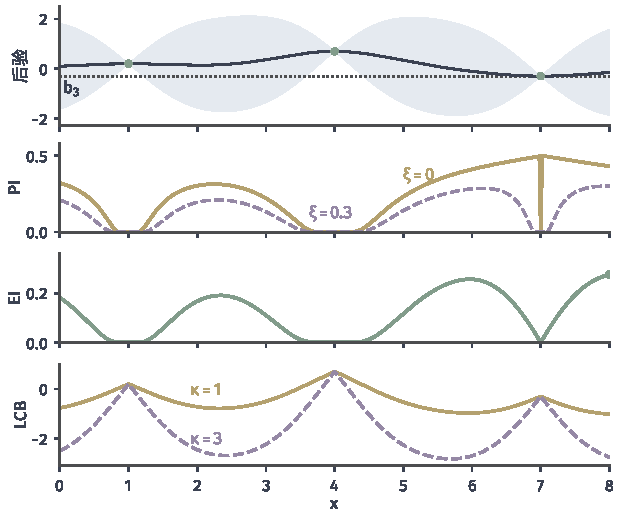
\includegraphics[width=105mm]{figures/05-optimization/05-stochastic-optimization/matplotlib/bo-acq-compare/figure.pdf}
 \caption{三种采集函数的比较，$t=3$，读数在$x=1,4,7$。第一行：深色线是后验均值，浅蓝带是均值上下两倍标准差，点线是$b_3$。第二行：改进概率，黄线$\xi=0$，紫虚线$\xi=0.3$。第三行：期望改进，绿点是最大点。第四行：置信下界，黄线$\kappa=1$，紫虚线$\kappa=3$，选点取最小点。}
 \label{fig:bo-acq-compare}
\end{BookInlineFigure}

\subsection{Thompson 采样}
\label{sec:bo-thompson}

前三种规则都把后验压缩成一个分数。\term{Thompson采样}（Thompson sampling）换了一种做法：不算分数，从当前后验抽取一整条函数$\widetilde{F}$，假装它就是真实目标，然后选它的最小点：
\begin{equation}
 \bm{x}_{t+1}\in\argmin_{\bm{x}\in\bm{C}}\widetilde{F}(\bm{x}),\qquad
 \widetilde{F}\sim F\mid\mathcal{D}_t.
 \label{eq:bo-thompson}
\end{equation}
一个位置被选中的概率，等于后验认为它是最小点的概率。乐观与谨慎不需要权重来调，而由后验分布本身决定：不确定的地方抽样起伏大，有机会被选中，但机会并不独占。

\paragraph{抽样要联合}
在有限候选集$\bm{x}_{1}',\ldots,\bm{x}_{N}'$上，抽样要从多元高斯分布$N(\bm{\mu},\bm{\Sigma})$抽取，$\bm{\mu}$和$\bm{\Sigma}$分别是后验均值向量和后验协方差矩阵。常用办法是作Cholesky分解$\bm{\Sigma}=\bm{L}\bm{L}^\top$，抽取标准正态向量$\bm{z}$，令
\begin{equation}
 \widetilde{\bm{F}}=\bm{\mu}+\bm{L}\bm{z}.
 \label{eq:bo-joint-sample}
\end{equation}

以$t=3$时的候选$x=6,8$为例。后验协方差矩阵和分解为
\[
 \bm{\Sigma}=\begin{bmatrix}0.746&-0.187\\-0.187&0.750\end{bmatrix},\qquad
 \bm{L}=\begin{bmatrix}0.864&0\\-0.217&0.838\end{bmatrix}.
\]
这里协方差是负的，这有一点反直觉：两点都与$x=7$相关，而$F(7)$已经确定，第~\ref{sec:bo-sequential}节会解释这个负号。

取$\bm{z}=(1,-0.5)^\top$，代入式~\eqref{eq:bo-joint-sample}，
\[
 \widetilde{F}(6)=-0.107+0.864=0.757,\quad
 \widetilde{F}(8)=-0.151-0.217-0.419=-0.787,
\]
这条样本的最小点在$x=8$。取$\bm{z}=(-1,0.5)^\top$，则
\[
 \widetilde{F}(6)=-0.971,\quad\widetilde{F}(8)=0.485,
\]
这条样本选$x=6$。两种结果都可能发生，选点因此带有随机性。

若把各点的边际分布独立抽样，得到的就不是后验函数。图~\ref{fig:bo-ts-paths}对比了在$0.1$网格上的两种抽样。(a)联合抽样是一条光滑曲线，穿过全部读数。(b)独立抽样忽略了相邻点的相关性，成了一串噪声，最小点总会落在方差最大的某处，这不是后验认为最可能的最小点。按20000条联合样本统计，最小点约四分之一的机会落在$x=8$附近，约四分之一的机会落在$x=6$附近，其余分散到$x=0$和$x=2$等位置。

\begin{BookInlineFigure}
 \centering
 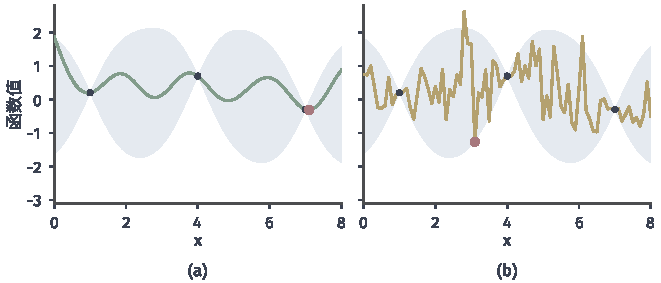
\includegraphics[width=112mm]{figures/05-optimization/05-stochastic-optimization/matplotlib/bo-ts-paths/figure.pdf}
 \caption{联合抽样与边际独立抽样。浅蓝带是$t=3$的后验均值上下两倍标准差，黑点是读数，红点是样本的最小点。(a)联合抽样得到的绿色曲线是一条可能的函数。(b)各网格点独立抽样得到的黄线不对应任何一条函数，把它的最小点当作选点并无依据。}
 \label{fig:bo-ts-paths}
\end{BookInlineFigure}

计算上，$N$个候选的联合抽样要作一次$O(N^3)$的分解。连续搜索域上不能抽取真正的无穷维函数，通常在较大的候选集上离散化，或用有限维随机特征近似，这些都是近似的来源。

\subsection{知识梯度（补充）}
\label{sec:bo-kg}

EI衡量的是“这次读数本身比现在最好的值低多少”。可是我们最终要交付的是推荐解，而一次读数即使本身不好，也可能让我们更清楚哪个位置该推荐。本小节换一个问题：这次观测能让最终推荐改善多少？

\paragraph{定义}
取一个推荐集合$\bm{R}\subseteq\bm{C}$，当前的最优推荐价值是后验均值的最小值$\min_{\bm{x}'\in\bm{R}}m_t(\bm{x}')$。设想在$\bm{x}$再观测一次，更新后的后验均值为$m_{t+1}$，它依赖尚未发生的读数，因而是随机的。\term{知识梯度}（knowledge gradient，KG）定义为
\begin{equation}
 \mathrm{KG}_t(\bm{x})=\min_{\bm{x}'\in\bm{R}}m_t(\bm{x}')-\mathbb{E}\Bigl[\min_{\bm{x}'\in\bm{R}}m_{t+1}(\bm{x}')\,\Bigm|\,\mathcal{D}_t,\bm{x}_{t+1}=\bm{x}\Bigr].
 \label{eq:bo-kg}
\end{equation}
更新后的均值以当前均值为期望，也就是
\[
 \mathbb{E}\bigl[m_{t+1}(\bm{x}')\mid\mathcal{D}_t\bigr]=m_t(\bm{x}').
\]
$\min$是凹函数，凹函数的期望不超过期望处的函数值（Jensen不等式），所以$\mathrm{KG}_t(\bm{x})\geq0$。

下一次读数的预测分布是$N(m_t(\bm{x}),s_t^2(\bm{x})+\tau^2)$，把标准化的预测残差记作$Z\sim N(0,1)$。把定理~\ref{thm:bo-posterior}应用于“以当前后验为先验、只含这一个观测”的情形，可得
\begin{equation}
 m_{t+1}(\bm{x}')=m_t(\bm{x}')+\widetilde{\sigma}_t(\bm{x}',\bm{x})Z,\quad
 \widetilde{\sigma}_t(\bm{x}',\bm{x})=\frac{c_t(\bm{x}',\bm{x})}{\sqrt{s_t^2(\bm{x})+\tau^2}}.
 \label{eq:bo-kg-update}
\end{equation}
每个推荐点的后验均值都随同一个$Z$线性移动，斜率取决于它与被观测位置的后验协方差。式~\eqref{eq:bo-kg}中的期望因此是一维积分，有限的$\bm{R}$上可以用分段线性包络精确算出，也可以用数值积分。

\paragraph{例：观测一个不推荐的位置}
取$\bm{R}=\{6,7\}$，当前后验均值$m_3(6)=-0.107$，$m_3(7)=-0.3$，当前最优推荐是$x=7$，价值$-0.3$。考虑观测$x=5$，它本身不在$\bm{R}$里。$x=7$已观测，$c_3(7,5)=0$，均值不动。由$c_3(6,5)\approx0.438$和$s_3(5)\approx0.864$，
\[
 \widetilde{\sigma}_3(6,5)\approx\frac{0.438}{0.864}\approx0.507.
\]

新的最优推荐价值是$\min\{-0.3,\ -0.107+0.507Z\}$。这个最小值可以写成$-0.3$减去$-0.3$与第二项之差的正部，代入式~\eqref{eq:bo-kg}，$\mathrm{KG}$恰好是阈值为$-0.3$的EI公式，只是均值和标准差换成$-0.107$与$0.507$：
\[
 \mathrm{KG}_3(5)\approx(-0.193)\Phi(-0.381)+0.507\,\phi(-0.381)\approx0.120.
\]
这个$x=5$的读数本身比$-0.3$低的可能性不大，因而$\mathrm{EI}_3(5)\approx0.117$，它的价值主要来自让我们更好地判断$x=6$。此处的KG同样不要求评价点属于$\bm{R}$，这是它与EI的不同，也允许最后推荐一个未曾评价的位置。

图~\ref{fig:bo-kg-vs-ei}比较了EI和取$\bm{R}$为$0.1$网格时的KG。两者的形状相近，但KG的最大点在$x\approx7.1$，紧靠当前最好点。在无噪声且核很光滑的模型中，贴着已知点再读一次，相当于测得该处的斜率，它能改变整段后验均值的最小位置，所以KG偏爱这里；而在恰好已观测的点上，读数不带来任何新信息，KG降为$0$，图中出现几个尖口。

\begin{BookInlineFigure}
 \centering
 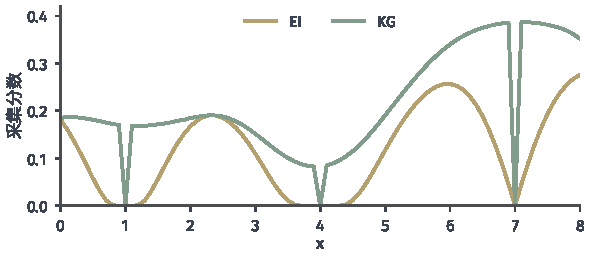
\includegraphics[width=100mm]{figures/05-optimization/05-stochastic-optimization/matplotlib/bo-kg-vs-ei/figure.pdf}
 \caption{EI与KG的对比，$t=3$，无噪声观测。黄线是期望改进，绿线是知识梯度（推荐集合为$0.1$网格，期望由$401$个等分位点数值积分）。KG在已观测点$x=1,4,7$上为$0$，在紧邻这些点的位置却不为$0$。}
 \label{fig:bo-kg-vs-ei}
\end{BookInlineFigure}

KG的计算比EI贵，并且对模型更敏感。一般的实验设计问题以信息价值安排观测，可参考\BookChapterRef{chap:observation-experiment-design}{卷八第9章“观测与实验设计”}；本章只把KG作为一种选点规则，在第~\ref{sec:bo-noisy}节有噪声时会再次用到它。

\section{顺序求解}
\label{sec:bo-sequential}

有了代理和采集函数，本节把它们接成一个完整的循环，回答一个具体问题：在预算$T$内，每一轮应当按什么次序做哪些计算，新读数又怎样改变下一轮的决策。

\paragraph{主要思想}
循环由两层组成，见图~\ref{fig:bo-loop}。外层是昂贵的真实评价，内层是便宜的计算：用数据建模，把模型转成分数，求分数的最大点。如果外层一次要几小时，内层花几秒钟算一个好的选点就很划算。

\begin{BookInlineFigure}
 \centering
 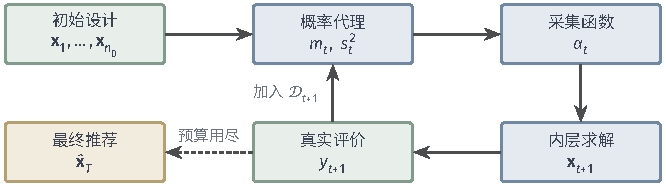
\includegraphics[width=112mm]{figures/05-optimization/05-stochastic-optimization/tikz/bo-loop/figure.pdf}
 \caption{贝叶斯优化的循环。绿框是需要运行真实目标的步骤，蓝框是只涉及代理模型的便宜计算，黄框是最后的输出。每轮读数加入$\mathcal{D}_{t+1}$，再回到概率代理更新。}
 \label{fig:bo-loop}
\end{BookInlineFigure}

每轮不必从头重算。第~\ref{sec:bo-posterior}节的后验本身是一个高斯过程，下一个读数相对它只是\emph{一个}新观测，把定理~\ref{thm:bo-posterior}应用于“以$(m_t,c_t)$为先验、只含一个观测”的情形，就得到更新式。记$\bm{x}^+=\bm{x}_{t+1}$，$y^+=y_{t+1}$，$v=s_t^2(\bm{x}^+)+\tau^2$，则
\begin{align}
 m_{t+1}(\bm{x})&=m_t(\bm{x})+\frac{c_t(\bm{x},\bm{x}^+)}{v}\bigl(y^+-m_t(\bm{x}^+)\bigr),
 \label{eq:bo-update-mean}\\
 c_{t+1}(\bm{x},\bm{x}')&=c_t(\bm{x},\bm{x}')-\frac{c_t(\bm{x},\bm{x}^+)\,c_t(\bm{x}',\bm{x}^+)}{v}.
 \label{eq:bo-update-cov}
\end{align}
式~\eqref{eq:bo-update-mean}说的是：新读数比预期低多少，其他位置就按它们与$\bm{x}^+$的后验协方差跟着调整多少，协方差为负的位置朝反方向调整。

\needspace{6\baselineskip}
\paragraph{变量}
贯穿例采用整数候选集，也就是把内层问题放在九个点上求解（内层的其他做法见第~\ref{sec:bo-inner}节）。计算中用到的量如下：
\begin{itemize}
 \item 已评价的位置与读数，长度为$t$的向量；
 \item 各候选点的后验均值$m_t$和后验协方差$c_t$，大小为$N\times N$，其中$N=9$；
 \item 当前最好值$b_t$；
 \item 每个候选点的采集分数，这里用EI。
\end{itemize}

\paragraph{初始化}
选取分散的初始点，运行真实评价，用定理~\ref{thm:bo-posterior}计算后验。例中初始点是$x=1,4,7$，读数$0.2,0.7,-0.3$，后验均值和标准差列在表~\ref{tab:bo-acq-values}中，$t=3$，$b_3=-0.3$。

\needspace{6\baselineskip}
\paragraph{每轮更新}
当$t<T$时，重复下面的步骤。
\begin{enumerate}
 \item \emph{计算采集分数。}对每个候选点按式~\eqref{eq:bo-ei}计算$\mathrm{EI}_t$。

 例中第一轮的分数见表~\ref{tab:bo-acq-values}，最大值$0.276$在$x=8$。

 \item \emph{选点并真实评价。}取分数最大的候选$\bm{x}^+$，运行目标，得到读数$y^+$。

 例中第一轮读到$f(8)=0.8$，比预期的$-0.151$高出很多，预测残差为
 \[
  y^+-m_3(8)\approx0.951.
 \]

 \item \emph{更新后验。}由式~\eqref{eq:bo-update-mean}和式~\eqref{eq:bo-update-cov}更新各候选点的均值和协方差，并更新$b_t$。

 例中$v=s_3^2(8)\approx0.750$，$c_3(6,8)\approx-0.187$，于是
 \[
  m_4(6)\approx-0.107+\frac{-0.187}{0.750}\times0.951\approx-0.345,
 \]
 \[
  s_4^2(6)\approx0.746-\frac{0.187^2}{0.750}\approx0.699.
 \]
 $x=6$的后验均值下降了，一次差的读数让另一个位置更有希望。由于$b_4$仍为$-0.3$，$\mathrm{EI}_4(6)$由$0.257$升到$0.356$，第二轮选$x=6$。
\end{enumerate}

$c_3(6,8)$的负号现在可以解释了。$x=6$和$x=8$都与$x=7$相关，而$F(7)$已知等于$-0.3$。在这个条件下，若$F(8)$比预期高，函数在$x=7$附近向右上升，光滑性要求它向左下降才能经过$F(7)$，于是$F(6)$偏低。

第二轮读到$f(6)=-1.0$，预测残差为$-0.655$，$v\approx0.699$，当前最好值变为$b_5=-1.0$。$x=5$与$x=6$的后验协方差$c_4(5,6)\approx0.431$，于是
\[
 m_5(5)\approx0.295+\frac{0.431}{0.699}\times(-0.655)\approx-0.109,
\]
\[
 s_5^2(5)\approx0.745-\frac{0.431^2}{0.699}\approx0.480.
\]

第三轮的分数变了样：$b_5$大幅降低，所有候选的EI都缩小了，
\[
 \mathrm{EI}_5(0)\approx0.042,\quad\mathrm{EI}_5(2)\approx0.037,\quad
 \mathrm{EI}_5(3)\approx0.020,\quad\mathrm{EI}_5(5)\approx0.032.
\]
EI选择了$x=0$，读到$f(0)=0.9$。此时$t=6=T$，预算用尽，循环结束。

最终得到的评价序列是$x=1,4,7,8,6,0$，读数最小的位置是$x=6$，推荐$\widehat{x}_6=6$，目标值$-1.0$。图~\ref{fig:bo-rounds}展示了三轮的后验和EI。第一轮两个峰高度相近；第二轮差读数把$x=6$的峰抬了起来；第三轮$b_t$下降后EI整体变小，算法转向还没有读数的左侧。

\begin{BookInlineFigure}
 \centering
 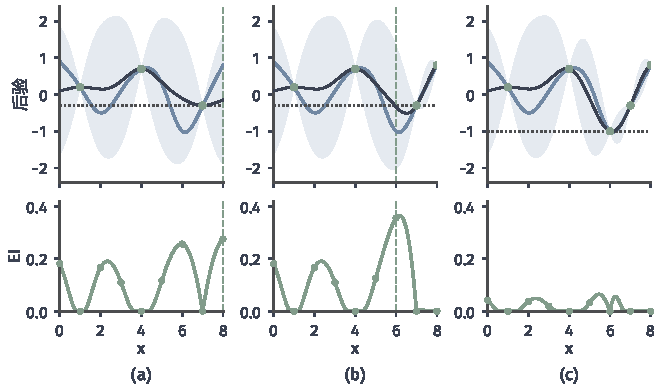
\includegraphics[width=112mm]{figures/05-optimization/05-stochastic-optimization/matplotlib/bo-rounds/figure.pdf}
 \caption{贯穿例的三轮选点。上行：蓝线是目标，深色线是后验均值，浅蓝带是均值上下两倍标准差，点线是当前最好值，绿点是读数。下行：绿线是EI，小点是整数候选上的分数。竖虚线是本轮选中的位置，依次为$x=8$、$x=6$、$x=0$。}
 \label{fig:bo-rounds}
\end{BookInlineFigure}

\subsection{初始设计}
\label{sec:bo-initial-design}

循环开始之前没有任何读数，采集函数没有依据（或者取决于先验，而先验下各处相同）。第一批点因此要在没有反馈的情况下放好，这一步称为\term{初始设计}（initial design）。本小节的问题是：放在哪里，放多少。

先验信息较少时，初始点的任务是覆盖搜索域的不同区域，同时为估计超参数提供不同间距的点对。图~\ref{fig:bo-initial-design}比较了单位方形上放九个点的三种办法。(a)均匀随机的点可能聚集，也可能在某些区域留白。(c)规则网格覆盖整齐，但投影到每个坐标上只有三个不同的值。(b)是\term{拉丁超立方抽样}（Latin hypercube sampling）：把每个坐标轴等分成九格，每行每列恰好放一个点，这样每个坐标轴的投影都分散。网格在高维时会失效，$n$维的$3^n$个格点很快超出预算。

\begin{BookInlineFigure}
 \centering
 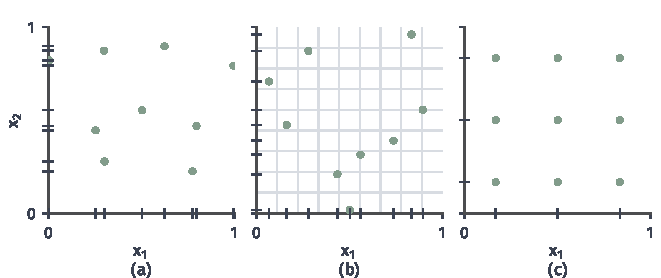
\includegraphics[width=112mm]{figures/05-optimization/05-stochastic-optimization/matplotlib/bo-initial-design/figure.pdf}
 \caption{单位方形上九个初始点的放置（固定随机种子）。(a)均匀随机；(b)拉丁超立方，浅灰线是九等分的格，每行每列恰好一个点；(c)规则网格。坐标轴上的短刻线是点在各坐标的投影，网格投影只有三个不同位置。}
 \label{fig:bo-initial-design}
\end{BookInlineFigure}

初始点不是越多越好，它们挤占后面的定向搜索。图~\ref{fig:bo-initial-budget}在贯穿例上固定总预算$T=8$，改变初始点数，其余用EI选点，统计$300$组随机初始点的平均终端误差。初始点不超过$4$时误差差别很小，因为这里的核是已知的，少量读数已经够用；初始点数达到$7$、$8$时，几乎没有定向评价的机会，平均误差升到$0.085$和$0.241$。

\begin{BookInlineFigure}
 \centering
 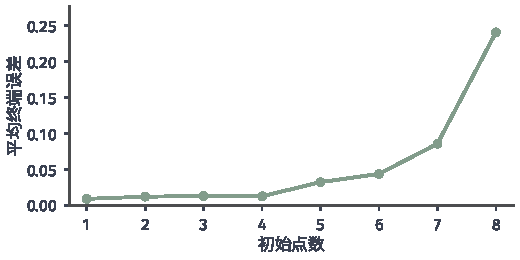
\includegraphics[width=88mm]{figures/05-optimization/05-stochastic-optimization/matplotlib/bo-initial-budget/figure.pdf}
 \caption{初始点数与最终效果。贯穿例，总预算$T=8$，初始点在$0.1$网格上均匀随机选取，其余用EI选点，纵轴是$300$组随机种子下的平均终端误差。初始点数等于$8$时全部预算都用于无反馈的覆盖。}
 \label{fig:bo-initial-budget}
\end{BookInlineFigure}

这个例子的核已知，所以很少的初始点就够了。核的超参数需要估计时，初始点太少会使边缘似然不可靠，代理在开始几轮可能严重失真，常见的经验是取搜索维数的若干倍（如$10n$），但这只是经验，总预算很小时要相应减少。

\subsection{采集函数求解}
\label{sec:bo-inner}

每轮要解一个内层优化问题：
\begin{equation}
 \bm{x}_{t+1}\in\argmax_{\bm{x}\in\bm{C}}\alpha_t(\bm{x}).
 \label{eq:bo-inner}
\end{equation}
它与外层目标的代价完全不同：$\alpha_t$是一个有解析式、可以快速求值的函数。但它一般不是凹函数，而且常有多个峰，本小节的问题就是怎样可靠地求它的最大点。

\paragraph{可用的导数}
真实目标不提供导数，但采集函数的导数完全来自代理。由式~\eqref{eq:bo-ei-derivatives}和链式法则，在$s_t(\bm{x})>0$的位置，
\begin{equation}
 \nabla\mathrm{EI}_t(\bm{x})=-\Phi(z)\nabla m_t(\bm{x})+\phi(z)\nabla s_t(\bm{x}).
 \label{eq:bo-ei-gradient}
\end{equation}
由式~\eqref{eq:bo-post-mean}和式~\eqref{eq:bo-post-cov}，令$\nabla\bm{k}_t(\bm{x})$表示$\bm{k}_t$对$\bm{x}$的Jacobi矩阵，并设核满足$k(\bm{x},\bm{x})$为常数，
\begin{align}
 \nabla m_t(\bm{x})&=\nabla\bm{k}_t(\bm{x})^\top\bm{A}_t^{-1}(\bm{y}_t-\bm{m}_{0,t})+\nabla m_0(\bm{x}),
 \label{eq:bo-grad-m}\\
 \nabla s_t(\bm{x})&=-\frac{\nabla\bm{k}_t(\bm{x})^\top\bm{A}_t^{-1}\bm{k}_t(\bm{x})}{s_t(\bm{x})}.
 \label{eq:bo-grad-s}
\end{align}
这些导数只要求核可导，不要求目标$f$可导。

用只有一个读数$F(7)=-0.3$的情形验算一下。取$x=6$，$b=-0.3$，则
\[
 k(6,7)=\tfrac12,\qquad \frac{\mathrm{d}k}{\mathrm{d}x}=-2\ln2\,(x-7)\,k\approx0.693.
\]
后验均值与方差及其导数是
\[
 m=-0.15,\quad m'\approx-0.208,\quad s\approx0.866,\quad s'\approx-0.400,
\]
其中$s'$由$(s^2)'=-2kk'$算得。这里$z\approx-0.173$，$\Phi(z)\approx0.431$，$\phi(z)\approx0.393$，代入式~\eqref{eq:bo-ei-gradient}，
\[
 \frac{\mathrm{d}\mathrm{EI}}{\mathrm{d}x}\approx0.431\times0.208-0.393\times0.400\approx-0.067.
\]
导数为负，说明从$x=6$向$x=7$走时，方差减小的损失超过了均值降低的收益。

\paragraph{多起点、候选筛选与随机搜索}
一个起点的局部上升只能到达它所在的峰。常用的做法是多起点局部优化：取一批起点，通常先在大量候选上计算$\alpha_t$，挑其中分数高的作起点，再用带约束的拟牛顿法作局部上升。也可以直接在候选集上比较分数，或用第~\ref{chap:random-search}章的随机搜索方法。这些方法都只求一个便宜函数的最大值，不增加昂贵评价。

图~\ref{fig:bo-inner-multistart}是贯穿例$t=5$时的情形。八个等距起点沿EI爬升，到达了四个不同的局部最大点，取值约为$0.042,0.049,0.065,0.057$，全局最大点在$x\approx5.46$。起点$x=7.5$附近EI几乎为零，梯度也几乎为零，上升根本走不动，这是平坦区域的常见困难，通常的对策是对EI取对数后再优化。

\begin{BookInlineFigure}
 \centering
 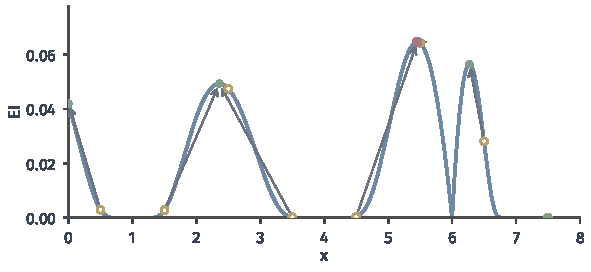
\includegraphics[width=100mm]{figures/05-optimization/05-stochastic-optimization/matplotlib/bo-inner-multistart/figure.pdf}
 \caption{内层问题的多起点求解。贯穿例$t=5$，蓝线是EI，黄色空心点是八个起点，灰色箭头是数值上升的起止，绿点是到达的局部最大点，红点是其中最好的点$x\approx5.46$。}
 \label{fig:bo-inner-multistart}
\end{BookInlineFigure}

对比这一轮的正文计算，整数候选集上的最大值是$\mathrm{EI}_5(0)\approx0.042$，而连续域上的最大点在$x\approx5.46$，取值$0.065$。内层问题的解法确实会改变外层的选点，这说明内层近似不是无关紧要的细节。内层近似求解也不自动得到采集函数的全局最优点；若分析某种算法的性质时假设了内层精确求解，实际运行时这个假设需要另外检查。

\subsection{观测更新}
\label{sec:bo-observation-update}

选定位置并运行真实评价之后，要回答的问题是：新读数应当怎样进入模型。

把新读数和它的噪声信息加入$\mathcal{D}_t$后，式~\eqref{eq:bo-update-mean}、式~\eqref{eq:bo-update-cov}更新候选点上的后验。若在搜索域的任意点上重新计算，需要更新Cholesky分解，也可以增量进行。设$\bm{A}_t=\bm{L}_t\bm{L}_t^\top$，新矩阵的因子只在末尾加一行：
\begin{equation}
 \bm{L}_{t+1}=\begin{bmatrix}\bm{L}_t&\bm{0}\\\bm{\ell}^\top&d\end{bmatrix},
 \label{eq:bo-chol-update}
\end{equation}
其中
\[
 \bm{\ell}=\bm{L}_t^{-1}\bm{k}_t(\bm{x}^+),\qquad
 d^2=k(\bm{x}^+,\bm{x}^+)+\tau^2-\bm{\ell}^\top\bm{\ell}.
\]
求$\bm{\ell}$只需一次前代，所以这一步需要$O(t^2)$次运算，不必花$O(t^3)$次重新分解。$d^2$恰好是新读数的预测方差$v$。如果这一轮重新估计了超参数，核矩阵整体改变，增量更新就不再适用，要重新分解。

这里要保留完整的历史，而不是只记住当前最好值。只记$b_t$的做法在第一轮之后只知道“最好值仍是$-0.3$”，看不到$x=8$的读数，也算不出$\mathrm{EI}_4(6)$从$0.257$升到$0.356$这个变化。未获改进的观测也有信息，它改变相关区域的预测，进而改变后续查询的价值。第一轮的$x=8$正是这种情形，图~\ref{fig:bo-rounds}(a)到(b)的变化说明了它的作用。

\section{含噪观测}
\label{sec:bo-noisy}

到目前为止，读数都是函数值本身。真实的仿真或实验常常带噪声，同一个$\bm{x}$运行两次，结果不一样。设
\begin{equation}
 y_i=f(\bm{x}_i)+\varepsilon_i,
 \label{eq:bo-noisy-obs}
\end{equation}
其中$\varepsilon_i$相互独立，服从均值为$0$、方差为$\tau^2$的高斯分布。此时要分清两个对象：未知但固定的函数值$f(\bm{x})$，和每次测量才产生的随机读数$y$。这就需要回答：噪声使前面哪些做法失效，选点规则应当怎样改？

\subsection{两种预测方差}
\label{sec:bo-noise-variances}

噪声出现后，“这个位置的不确定性”有两种说法。一种是对潜在函数值$F(\bm{x})$的不确定，后验方差为$s_t^2(\bm{x})$。另一种是对下一次读数$y$的不确定，这要多加一份测量噪声。独立噪声方差为$\tau^2$时，
\begin{equation}
 \operatorname{Var}(y\mid\mathcal{D}_t,\bm{x})=s_t^2(\bm{x})+\tau^2.
 \label{eq:bo-pred-var}
\end{equation}
这里用到$y=F(\bm{x})+\varepsilon$，新的$\varepsilon$与$F$及已有数据独立，方差相加。

图~\ref{fig:bo-noise-bands}展示了两者的差别。浅蓝带表示潜在函数值的范围，紫色虚线表示下一次读数可能的范围。读数点不再落在后验均值上，模型会把读数“往回拉”，因为它知道读数里含有噪声；即使在读数附近，后验方差也不为零。

\begin{BookInlineFigure}
 \centering
 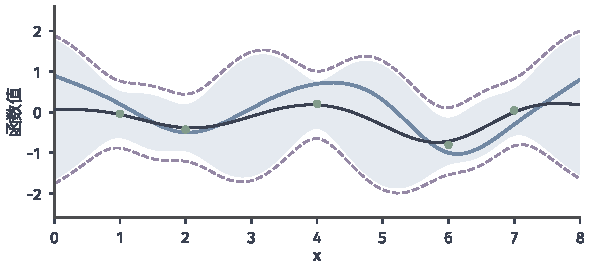
\includegraphics[width=100mm]{figures/05-optimization/05-stochastic-optimization/matplotlib/bo-noise-bands/figure.pdf}
 \caption{两种预测方差。噪声标准差$\tau=0.3$，绿点是五个含噪读数（固定随机种子）。蓝线是目标，深色线是后验均值，浅蓝带是$m_t\pm2s_t$，紫虚线是$m_t\pm2\sqrt{s_t^2+\tau^2}$。}
 \label{fig:bo-noise-bands}
\end{BookInlineFigure}

在同一位置重复读数，能减少的是第一种方差。设先验方差为$1$，$\tau^2=0.09$，在$x$处读$n$次，由定理~\ref{thm:bo-posterior}，
\[
 s^2(x)=\frac{\tau^2}{n+\tau^2}.
\]
$n=1,4,9$时，$s^2$依次约为
\[
 0.083,\qquad 0.022,\qquad 0.010.
\]
而下一次读数的方差始终比$s^2$多$0.09$，这一份噪声不会因观测而消失。观测多了，我们越来越清楚$f(x)$是多少，但下一次测量出来的数照样抖动。

\paragraph{方差能否只减不增}
超参数固定时，由更新式~\eqref{eq:bo-update-cov}，
\[
 s_{t+1}^2(\bm{x})=s_t^2(\bm{x})-\frac{c_t(\bm{x},\bm{x}^+)^2}{s_t^2(\bm{x}^+)+\tau^2}\leq s_t^2(\bm{x}),
\]
新增观测不会使潜在值的后验方差增大。这个结论只在模型固定时成立。

重新拟合超参数就可能使方差增大。设$k=\sigma^2k_0$，其中$k_0$是贯穿例的核，幅度$\sigma^2$用边缘似然估计，无噪声。只有$x=1$的读数$1$时，估计值$\widehat{\sigma}^2=1$，于是
\[
 s^2(2)=\widehat{\sigma}^2\cdot\tfrac34=0.75.
\]
再评价相距很远的$x=6$，读到$3$，两点几乎不相关，幅度估计变为
\[
 \widehat{\sigma}^2\approx\frac{1^2+3^2}{2}=5,
\]
于是$s^2(2)\approx3.75$，反而变大了。新读数告诉模型“函数的波动比原来以为的大”，模型便下调了之前的把握。这两种情形都和“消除下一次测量的噪声”无关。

\subsection{含噪选点}
\label{sec:bo-noisy-selection}

\paragraph{最低读数可能只是运气好}
式~\eqref{eq:bo-incumbent}的$b_t$在含噪时不能直接用读数的最小值代替。读数的最小值常常是噪声偏向负方向的那一次。图~\ref{fig:bo-noise-incumbent}上半部分中，六个读数里最低的是$x=2$处的$-0.95$（红圈），但$f(2)=-0.5$，真实更好的$x=6$只读到$-0.55$，因为那次噪声是正的。

用含噪的最低读数做阈值，会把门槛设得过低，好像已经找到一个其实并不存在的好结果。一种改法是把阈值换成已评价点上的最小后验均值，这样噪声被模型部分平滑了；这是一种具体的近似规则，并不等于对真实阈值作了正确处理。

\paragraph{含噪期望改进}
更一致的做法是承认阈值也不确定。真实的“已评价最好值”是$\min_iF(\bm{x}_i)$，它是随机的。把它和候选点放在同一个后验下，定义\term{含噪期望改进}（noisy expected improvement，NEI）：
\begin{equation}
 \mathrm{NEI}_t(\bm{x})=\mathbb{E}\Bigl[\bigl(\min_{i\leq t}F(\bm{x}_i)-F(\bm{x})\bigr)_+\,\Bigm|\,\mathcal{D}_t\Bigr].
 \label{eq:bo-nei}
\end{equation}
这里的期望对$F(\bm{x}_1),\ldots,F(\bm{x}_t),F(\bm{x})$的\emph{联合}后验取，协方差不能丢：若候选点与某已评价点强相关，两者的差就不会太大。一般情形下没有闭式，常用的做法是抽取这$t+1$个值的联合后验样本，取平均。

\paragraph{例：只有一个评价点}
只有一个评价点时，NEI可以手算。设$\tau^2=0.09$，在$x=2$读到$y=-0.5$，候选为$x=4$。相关系数$\rho=1/16$，由定理~\ref{thm:bo-posterior}，
\[
 \begin{aligned}
 F(2)\mid\mathcal{D}:&\ \text{均值}\ -0.459,\quad\text{方差}\ 0.083,\\
 F(4)\mid\mathcal{D}:&\ \text{均值}\ -0.029,\quad\text{方差}\ 0.996,
 \end{aligned}
\]
两者的后验协方差约为$0.005$。

把$D=F(2)-F(4)$看成一个高斯量，其均值与方差为
\[
 \mathbb{E}D\approx-0.430,\qquad \operatorname{Var}D\approx0.083+0.996-2\times0.005\approx1.069.
\]
由于$\mathrm{NEI}=\mathbb{E}D_+$，用式~\eqref{eq:bo-ei}的同一积分，标准化后$u\approx-0.416$，
\[
 \mathrm{NEI}\approx-0.430\,\Phi(u)+1.034\,\phi(u)\approx0.233.
\]

同一位置上，以读数$-0.5$为阈值的EI约为$0.206$，以后验均值$-0.459$为阈值的EI约为$0.220$。NEI最大，因为它考虑了阈值$F(2)$自身的不确定性：阈值可能比后验均值高，候选点就更容易改进。

图~\ref{fig:bo-noise-incumbent}下半部分比较了三种做法。阈值用最低读数时，门槛被噪声压低，除$x=2$附近外，分数都比另外两条线小（黄线）；阈值用最小后验均值时，$x=2$处仍有一个较高的峰，因为最小后验均值落在$x=2$（紫虚线）；NEI在已评价的$x=2$附近凹下去，并把价值分到其他地方（绿线）。

\begin{BookInlineFigure}
 \centering
 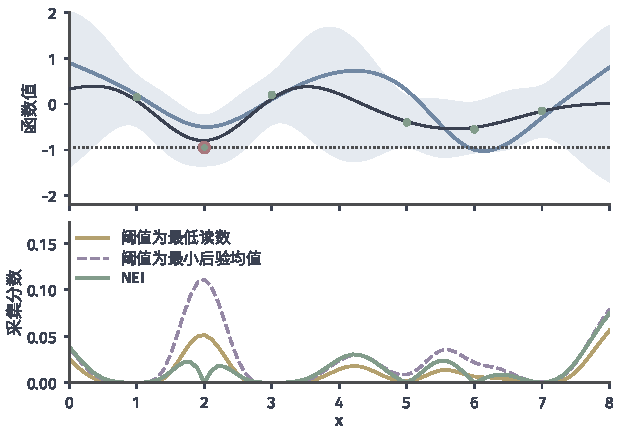
\includegraphics[width=105mm]{figures/05-optimization/05-stochastic-optimization/matplotlib/bo-noise-incumbent/figure.pdf}
 \caption{最低读数与含噪选点。上：$\tau=0.3$，六个读数，噪声依次取为$-0.05,-0.45,0.1,-0.7,0.45,0.15$（手工给定，用以突出$x=2$的偶然低值），红圈是最低读数，点线是其数值；蓝线是目标，深色线是后验均值。下：三种采集分数，NEI由$40000$个联合后验样本估计。}
 \label{fig:bo-noise-incumbent}
\end{BookInlineFigure}

NEI和知识梯度衡量的东西不同。NEI问的是“潜在函数值能否低于已评价点”，KG问的是“这次观测后，最终推荐的价值能改善多少”。无噪声时前者是EI的直接推广，后者需要再做一次前瞻。两者都在含噪时有定义，下一节就会看到它们对“重复测量”的回答相反。

\subsection{重复评价}
\label{sec:bo-replicates}

含噪时一个自然的动作是把同一个位置再测一次。这样做有用吗？按潜在改进的定义，答案是否定的。若$\bm{x}$恰好是某个已评价点$\bm{x}_j$，则$\min_iF(\bm{x}_i)\leq F(\bm{x}_j)$，改进量恒为$0$，所以
\begin{equation}
 \mathrm{NEI}_t(\bm{x}_j)=0.
 \label{eq:bo-nei-zero}
\end{equation}
图~\ref{fig:bo-noise-incumbent}的绿线在$x=2$处贴到零，正是这个原因。NEI从定义上就看不到复测的价值，因为复测不产生新位置，只是更清楚地认识旧位置。

复测的价值要由信息更新的准则来衡量。式~\eqref{eq:bo-kg}的KG没有这种限制。设两个候选A、B，$F(\text{A})$的后验均值$0$，方差$s^2=0.04$，$F(\text{B})$的后验均值$0.1$，两者后验独立，测量噪声$\tau^2=0.09$。当前推荐A。再测一次A后，由式~\eqref{eq:bo-kg-update}，
\[
 \widetilde{\sigma}=\frac{0.04}{\sqrt{0.04+0.09}}\approx0.111.
\]

新的推荐价值是$\min\{0.111Z,\ 0.1\}$，标准化的间距$u=0.1/0.111\approx0.901$。于是
\[
 \begin{aligned}
 \mathrm{KG}&=0-\mathbb{E}\min\{0.111Z,\,0.1\}\\
 &=0.111\bigl(\phi(u)-u(1-\Phi(u))\bigr)\approx0.011.
 \end{aligned}
\]
这个值大于$0$：再测一次A可能发现它其实比B差，从而改变推荐。

\paragraph{该重复多少次}
重复次数取决于要区分的差距和噪声。设两个候选的真实差距为$\Delta$，噪声标准差为$\tau$，各读$n$次后比较平均读数，选对的概率为
\begin{equation}
 \mathbb{P}(\text{选对})=\Phi\left(\frac{\Delta\sqrt{n}}{\tau\sqrt{2}}\right).
 \label{eq:bo-correct-selection}
\end{equation}
这里用到两个平均读数之差服从$N(\Delta,2\tau^2/n)$。取$\Delta=0.2$，$\tau=0.3$，$n=1,4,9$时的概率依次为
\[
 0.681,\qquad 0.827,\qquad 0.921.
\]
可见差距接近噪声水平时，一次测量基本在碰运气。代价接近的候选之间要靠复测来决定，能否负担这个复测要由预算决定。

最后要留意单次异常读数。一个比预期低$3$倍标准差的读数，可能是噪声，也可能是模型错了，比如该位置附近有一个模型没想到的窄谷。留一残差~\eqref{eq:bo-loo}只能发现它异常，不能告诉我们原因。在同一位置复测可以帮助区分：回到预期附近，说明是噪声；复测仍然很低，说明应当修改模型的设定。

\section{约束下的选点}
\label{sec:bo-constraints}

前面的搜索域是已知的。实际问题常带约束，其中有两类要分开。已知且容易判断的约束，比如参数上下限、整数限制，在内层问题~\eqref{eq:bo-inner}里直接限定搜索域即可，真实评价都发生在可行点上。另一类是未知且昂贵的约束：例如“峰值应力不超过上限”，只有仿真运行结束才知道是否满足。

设目标损失和性能上限都要运行才能测得，问题写成
\begin{equation}
 \min_{\bm{x}\in\bm{C}}\ f(\bm{x})\quad\text{s.t.}\quad g_j(\bm{x})\leq0,\ \ j=1,\ldots,m.
 \label{eq:bo-constrained}
\end{equation}
一个候选点的目标值可以很好，却是不可行的。怎样让未知约束进入选点，而“最终可行”和“每次试验都可行”又有什么不同？

\subsection{可行概率}
\label{sec:bo-feasibility}

对每个$g_j$也用一个代理建模，得到后验$G_j$。候选点满足全部约束的后验概率称为可行概率。若当前后验下各约束相互独立，并且第$j$个约束的后验为$N(m_j(\bm{x}),s_j^2(\bm{x}))$，$s_j(\bm{x})>0$，则
\begin{equation}
 \mathrm{PF}_t(\bm{x})=\prod_{j=1}^m\Phi\left(\frac{-m_j(\bm{x})}{s_j(\bm{x})}\right).
 \label{eq:bo-feasible-prob}
\end{equation}

阈值$b_t$也要相应改变：它是已评价点中\emph{可行者}的最好读数。一个不可行点读数再低，也不能作为改进的基准。可行改进的期望是
\[
 \mathbb{E}\Bigl[\bigl(b_t-F(\bm{x})\bigr)_+\,\mathbf{1}\{G_j(\bm{x})\leq0,\ \forall j\}\,\Bigm|\,\mathcal{D}_t\Bigr].
\]
其中$\mathbf{1}\{\cdot\}$表示事件成立时取$1$、否则取$0$。

当前后验下，目标改进与各约束事件相互独立时，乘积的期望等于期望的乘积，所以
\begin{equation}
 \mathrm{cEI}_t(\bm{x})=\mathrm{EI}_t(\bm{x})\cdot\mathrm{PF}_t(\bm{x}).
 \label{eq:bo-cei}
\end{equation}
独立这个条件不能省略。若目标和约束由同一个物理量驱动，相关性强，式~\eqref{eq:bo-cei}就不再是可行改进的期望，需要联合积分。

\paragraph{贯穿例}
在贯穿例上加一个约束$g(x)=(x-4.5)/4\leq0$，算法只能通过评价得知它的值，用同样的核建模。三个读数为$g(1)=-0.875$，$g(4)=-0.125$，$g(7)=0.625$。$x=7$不可行，尽管它读数最低，因此可行最好值是
\[
 b_3=f(1)=0.2.
\]

计算$x=2$的$\mathrm{cEI}$。目标的后验$m=0.143$，$s=0.864$，代入式~\eqref{eq:bo-ei}得$\mathrm{EI}\approx0.374$。约束的后验$m_g\approx-0.445$，$s_g\approx0.864$，可行概率为
\[
 \Phi(0.445/0.864)=\Phi(0.515)\approx0.697.
\]
于是
\[
 \mathrm{cEI}(2)\approx0.374\times0.697\approx0.261.
\]

表~\ref{tab:bo-cei}列出几个候选的结果。不考虑约束的EI选择$x=8$，加上可行概率之后，右侧候选的分数大幅下降，最大值转到$x=0$。图~\ref{fig:bo-constrained}画出了完整的曲线：$x=7$的EI是$0.5$，但$g(7)>0$已知，cEI为$0$。

\begin{BookInlineTable}
 \centering
 \caption{贯穿例的约束选点，$t=3$，$b_3=0.2$（可行读数中最小的）。}
 \label{tab:bo-cei}
 \begin{tabular}{cccccc}
 \toprule
 $x$&$\mathrm{EI}$&$m_g$&$s_g$&$\mathrm{PF}$&$\mathrm{cEI}$\\
 \midrule
 0&0.398&$-0.437$&0.866&0.693&$\mathbf{0.276}$\\
 2&0.374&$-0.445$&0.864&0.697&0.261\\
 6&0.520&0.305&0.864&0.362&0.188\\
 8&0.549&0.313&0.866&0.359&0.197\\
 \bottomrule
 \end{tabular}
\end{BookInlineTable}

\begin{BookInlineFigure}
 \centering
 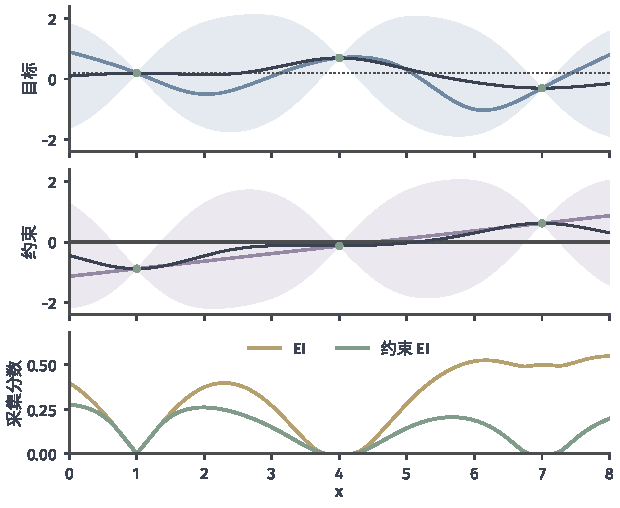
\includegraphics[width=105mm]{figures/05-optimization/05-stochastic-optimization/matplotlib/bo-constrained/figure.pdf}
 \caption{未知约束下的选点。上：目标的后验，蓝线是目标，点线是当前可行最好值$b_3=0.2$。中：约束的后验，紫线是真实的$g$，深灰线是边界$g=0$。下：黄线是不考虑约束的EI，绿线是约束EI，$x=7$处EI较大但已知不可行，约束EI为$0$。}
 \label{fig:bo-constrained}
\end{BookInlineFigure}

\paragraph{还没有可行点时}
读数中若没有可行点，$b_t$没有定义，EI也就无从算起。这时需要先规定一个寻找可行点的准则，最常见的是选$\mathrm{PF}_t(\bm{x})$最大的位置，等找到第一个可行点后，再转入$\mathrm{cEI}$。

\subsection{评价的可行性}
\label{sec:bo-eval-feasibility}

约束有两种含义，到这里还没有分开：一种要求\emph{最终推荐解}可行，中途的试验可以不可行；另一种要求\emph{每次试验}都不能违反约束，比如试验中的设备一旦过热就会损坏。前面的$\mathrm{cEI}$只处理第一种，它会故意到不可行区域采样，以弄清边界。

第二种要求要严格得多。单个点的后验可行概率高并不够用。设每轮选的点可行概率都是$0.95$，假设各轮近似独立，$20$轮全部可行的概率只有
\[
 0.95^{20}\approx0.36.
\]
要保证每次试验都可行，需要三样额外的东西：能把模型与真实约束联系起来的假设（例如$g$确实来自这个高斯过程，或有已知的Lipschitz常数）、至少一个已知可行的初始点、以及保守的选点规则。

图~\ref{fig:bo-safe-set}展示了一种保守的做法：以$g$的后验上界$m_g+2s_g\leq0$定义\emph{安全集}，每轮只在安全集内选点，示例中都取安全集的右端点。这里的约束是前面的$g(x)=(x-4.5)/4$，初始已知$x=1$可行。安全集三轮依次为
\[
 [0.66,1.34],\qquad[0.48,1.76],\qquad[0.32,2.28].
\]
这样的扩张靠边界附近的试验逐步推进，很慢，也可能永远到不了与初始点隔开的另一块可行区域。而且上界中的系数$2$是单点意义上的；要保证所有试验都安全，系数还须按第~\ref{sec:bo-guarantees}节的方式放大。

\begin{BookInlineFigure}
 \centering
 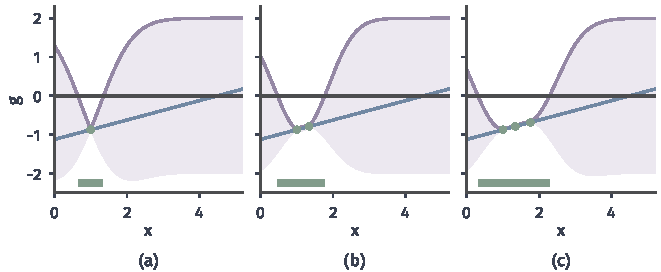
\includegraphics[width=112mm]{figures/05-optimization/05-stochastic-optimization/matplotlib/bo-safe-set/figure.pdf}
 \caption{保守选点下安全集的扩张。蓝线是真实约束$g(x)=(x-4.5)/4$，深灰线是边界，浅紫带是后验$m_g\pm2s_g$，紫线是上界$m_g+2s_g$，绿点是已做的试验，底部绿色粗线是上界不超过$0$的安全集。(a)、(b)、(c)依次是第一、二、三轮。}
 \label{fig:bo-safe-set}
\end{BookInlineFigure}

\section{批量评价}
\label{sec:bo-batch}

到现在为止，算法一次只运行一个试验，等结果回来再决定下一个。如果手上有两台机器，就可以同时跑两个。于是要问：多个试验同时运行时，候选应当怎样选，尚未返回的试验又该如何处理？

并行带来的好处和代价都很具体。图~\ref{fig:bo-parallel-timeline}比较了完成四次评价的三种方式。(a)一台机器逐个运行，每次选点都能用上之前全部结果，总时长最长。(b)两台机器同步批量运行，时长减半，但第$2$次评价没有用上第$1$次的结果。(c)两台机器异步运行，耗时不等，一台空出来就立刻派新试验，此时另一台上的试验还没有结果。

\begin{BookInlineFigure}
 \centering
 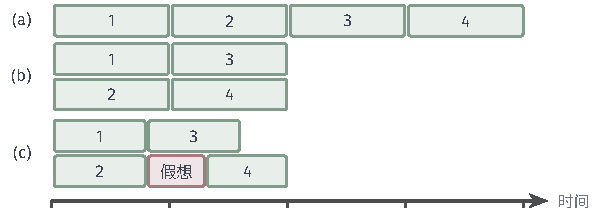
\includegraphics[width=102mm]{figures/05-optimization/05-stochastic-optimization/tikz/bo-parallel-timeline/figure.pdf}
 \caption{四次评价的三种安排，横轴是时间，每个绿框是一次评价，数字是选点顺序。(a)串行。(b)两台机器的同步批量。(c)异步，两台机器上的评价耗时不等，第$3$次选点时第$2$次评价还在运行，第$2$次评价后段的红框表示这段时间里结果尚未返回，第$3$次选点的计算对它使用假想结果，它不是观测。}
 \label{fig:bo-parallel-timeline}
\end{BookInlineFigure}

\subsection{联合选点}
\label{sec:bo-joint-batch}

一次选$q$个点时，最容易想到的做法是取单点采集分数最高的$q$个位置。问题在于这$q$个点常常挤在一个峰上。图~\ref{fig:bo-batch-joint}是贯穿例$t=4$时、在$0.25$网格上选两点的结果：单点EI最高的两点是$x=6.25$和$x=6$（黄方块），它们几乎重复。

应当衡量的是整批的价值。无噪声时，一批候选$\bm{x}_1',\ldots,\bm{x}_q'$的批量期望改进（q-EI）是
\begin{equation}
 \mathrm{qEI}_t(\bm{x}_1',\ldots,\bm{x}_q')=\mathbb{E}\Bigl[\bigl(b_t-\min_{j\leq q}F(\bm{x}_j')\bigr)_+\,\Bigm|\,\mathcal{D}_t\Bigr].
 \label{eq:bo-qei}
\end{equation}
期望对这$q$个函数值的联合后验取，所以候选点之间的相关性直接影响整批的价值。

\paragraph{相关性怎样影响整批价值}
用两个候选说清楚。设$b_t=0$，两者的后验均为$N(0,1)$，相关系数为$\rho$。单点EI都是$\phi(0)\approx0.399$，这里记$X=-F(\bm{x}_1')$，$Y=-F(\bm{x}_2')$，则
\[
 \mathrm{qEI}=\mathbb{E}\max\{0,X,Y\}.
\]

三个数$0,X,Y$从小到大排列为$U_1\leq U_2\leq U_3$。对$a,b,c$两两取最大值再求和，结果等于最大数的两倍加中间数，所以
\[
 2U_3+U_2=\max\{0,X\}+\max\{0,Y\}+\max\{X,Y\}.
\]

$(X,Y)$与$(-X,-Y)$同分布，取负号后最小的变成最大的，中间的仍是中间的，并且符号相反，所以$\mathbb{E}U_2=0$。两边取期望，再用
\[
 \mathbb{E}\max\{0,X\}=\frac1{\sqrt{2\pi}},\qquad
 \mathbb{E}\max\{X,Y\}=\sqrt{\frac{1-\rho}{\pi}},
\]
其中第二式来自$\max\{X,Y\}=(X+Y+\lvert X-Y\rvert)/2$和$X-Y\sim N(0,2(1-\rho))$，得到
\begin{equation}
 \mathrm{qEI}=\frac1{\sqrt{2\pi}}+\frac12\sqrt{\frac{1-\rho}{\pi}}.
 \label{eq:bo-qei-two}
\end{equation}

取$\rho=1,0.5,0$时，$\mathrm{qEI}$依次约为
\[
 0.399,\qquad 0.598,\qquad 0.681.
\]
两点完全相同时，第二个点没有价值，整批的价值就是单点EI；越不相关，第二个点带来的额外机会越大。但即使独立，第二个点的边际价值也小于单点EI的$0.399$，因为它和第一个点要竞争同一个“成为更好者”的位置。所以把单点分数相加不等于整批的价值。

回到贯穿例。单点EI最高的两点，整批$\mathrm{qEI}\approx0.407$，两点的单点EI之和却是$0.719$。$0.25$网格上最好的一对是$x=2.25$和$x=6.25$（绿点），整批$\mathrm{qEI}\approx0.487$，第二个点不再去挤第一个峰。

\begin{BookInlineFigure}
 \centering
 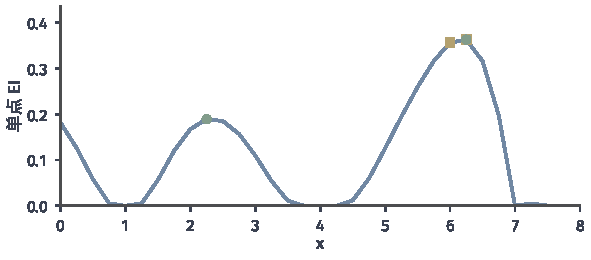
\includegraphics[width=100mm]{figures/05-optimization/05-stochastic-optimization/matplotlib/bo-batch-joint/figure.pdf}
 \caption{一次选两点。贯穿例$t=4$，$0.25$网格，蓝线是单点EI。黄方块是单点分数最高的两点（$x=6$与$x=6.25$），绿点是使$\mathrm{qEI}$最大的两点（$x=2.25$与$x=6.25$），后者由$40000$个公共后验样本估计，$x=6.25$的绿点与黄方块重合。}
 \label{fig:bo-batch-joint}
\end{BookInlineFigure}

$q$大时联合优化是$qn$维的内层问题，闭式也不再存在，通常用联合样本近似期望，再用重参数化式~\eqref{eq:bo-joint-sample}对候选位置求梯度。

\subsection{未完成的评价}
\label{sec:bo-pending}

异步运行时，一台机器空出来要立刻派新试验，而另一台上的试验还没有结果。本小节的问题是：尚未返回的试验，在选点计算中该如何对待。

忽略它们不对。忽略后下一轮的选择可能恰好与运行中的位置重复。图~\ref{fig:bo-pending-fantasy}中，若$x=6$的试验正在运行，黄线仍在$x=6$处给出高分。把运行中的位置也算作数据，就要用读数，而读数还没有。

正确做法是对可能的结果作平均。设运行中的位置为$\bm{x}_{\mathrm{p}}$，结果按当前预测分布取值，定义
\begin{equation}
 \bar\alpha_t(\bm{x})=\mathbb{E}_{y_{\mathrm{p}}}\bigl[\alpha_t\bigl(\bm{x}\mid\mathcal{D}_t\cup\{(\bm{x}_{\mathrm{p}},y_{\mathrm{p}})\}\bigr)\bigr],
 \label{eq:bo-fantasy}
\end{equation}
其中期望按$y_{\mathrm{p}}\sim N(m_t(\bm{x}_{\mathrm{p}}),s_t^2(\bm{x}_{\mathrm{p}})+\tau^2)$计算，实际常用少量抽样近似。

这里用于计算的$y_{\mathrm{p}}$称为假想结果，它不是观测，不能写进$\mathcal{D}_t$，算完就丢弃。真实结果返回后，仍须用真实读数更新后验。

看$\bm{x}_{\mathrm{p}}=6$的情形（无噪声，$t=3$）。对任何假想结果，$x=6$处的后验方差都变为零，改善量都是$0$，平均之后$\bar\alpha_3(6)=0$。图中绿线在$x=6$降到零，附近也被压低，$x=8$的分数从$0.276$降到约$0.233$，因为阈值在有些假想情形下变低了。这样下一台机器不会与运行中的试验重复。

\begin{BookInlineFigure}
 \centering
 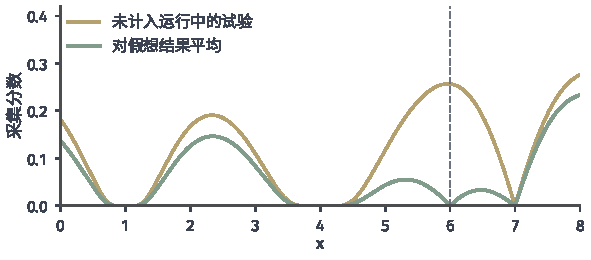
\includegraphics[width=100mm]{figures/05-optimization/05-stochastic-optimization/matplotlib/bo-pending-fantasy/figure.pdf}
 \caption{对运行中试验的处理。贯穿例$t=3$，竖虚线是运行中的位置$x=6$。黄线是不考虑运行中试验的EI，绿线是对假想结果取平均之后的EI（$201$个等分位假想读数）。绿线在$x=6$处为$0$。}
 \label{fig:bo-pending-fantasy}
\end{BookInlineFigure}

\section{预算与结果评价}
\label{sec:bo-budget}

循环总要结束。本节回答最后几个问题：预算究竟应当怎样计算，什么时候停止，交出什么，这个结果好到什么程度，以及哪些结论有理论保证。这些问题放在一起，是因为比较方法时必须固定同一套口径：搜索域、可用信息和预算。

\subsection{评价成本}
\label{sec:bo-cost}

不同位置的运行代价可能差别很大，比如某个参数越大，仿真越慢。一种常见的调整是除以预测成本$\widehat{c}(\bm{x})$，选单位成本的改进最大的点：
\begin{equation}
 \alpha_t^{\mathrm{cost}}(\bm{x})=\frac{\mathrm{EI}_t(\bm{x})}{\widehat{c}(\bm{x})}.
 \label{eq:bo-cost-ei}
\end{equation}
这只是一种特定的预算策略，它不自动最优地分配剩余总预算。下面的小例子说明这一点。剩余预算是$9$，候选A成本$1$、预期收益$2$，候选B成本$9$、预期收益$16.2$。单位成本的收益分别为
\[
 2,\qquad1.8.
\]
按单位成本选A，用掉$1$后，剩余$8$不够运行B，总收益只有$2$；一开始就选B，总收益为$16.2$。贪心比值没有考虑“预算够不够下一个”。

时间也要分开算。评价次数少不等于总耗时短。表~\ref{tab:bo-time}区分三种常被混用的时间。若一次评价只要$1$秒，贝叶斯优化的内层计算可能远超评价本身，这时随机搜索更快；若一次评价要$1$小时，每轮花$1$分钟做选点几乎没有成本。比较方法时只比较外层迭代数，等于默认了内层计算不要钱。

\begin{BookInlineTable}
 \centering
 \caption{三种时间口径，$c_i$是第$i$次评价的耗时，$a_i$是第$i$轮算法计算的耗时，$q$是并行的机器数。}
 \label{tab:bo-time}
 \begin{tabular}{ll}
 \toprule
 口径&计算方式\\
 \midrule
 串行总耗时&$\sum_i(c_i+a_i)$\\
 并行等待时间&约$\sum_i c_i/q$，耗时不等时更长\\
 算法自身计算时间&$\sum_i a_i$，高斯过程每轮约$O(t^3)$\\
 \bottomrule
 \end{tabular}
\end{BookInlineTable}

\subsection{停止与推荐}
\label{sec:bo-stopping}

最直接的停止条件是预算耗尽，这不需要任何模型。也可以在采集分数很小时提前停止，例如$\max_{\bm{x}}\mathrm{EI}_t(\bm{x})$低于一个阈值。这种停止依赖两件事：代理是否可信，以及内层求解是否找到了采集函数的最大点。第~\ref{sec:bo-model-specification}节中$\ell=3$的模型在$x=6$处方差极小，据此计算的EI也很小，算法就会在没有真正探索的情况下停下来。

推荐规则要在运行前说定。无噪声时可以返回已评价的最好点，贯穿例中就是$\widehat{x}_6=6$。含噪时，已评价的最好读数可能只是运气，通常用后验均值提出候选，例如选$\min_{\bm{x}}m_T(\bm{x})$的位置，再用预留的预算在候选处复测。最后报告采用的推荐规则，以及推荐值的不确定性，不只报告一个数字。

\subsection{推荐误差}
\label{sec:bo-regret}

交出$\widehat{\bm{x}}_T$后，自然要问它离最好的结果有多远。记$f^\star=\inf_{\bm{x}\in\bm{C}}f(\bm{x})$，用\term{简单遗憾}（simple regret）$f(\widehat{\bm{x}}_T)-f^\star$衡量最终结果，也就是终端的推荐误差。

另一个常见的量是\term{累积遗憾}（cumulative regret）：
\begin{equation}
 R_T=\sum_{t=1}^T\bigl(f(\bm{x}_t)-f^\star\bigr).
 \label{eq:bo-cumulative-regret}
\end{equation}
它把每次评价相对$f^\star$的损失都算进去，适用于每次试验本身就有代价的场合，这种在线损失的完整讨论可参考\BookChapterRef{chap:partial-observation-exploration}{卷十第3章“部分观测、主动观测与探索”}。两者回答的问题不同：贝叶斯优化的目标是最后交一个好答案，探索阶段的差读数并不算损失。

贯穿例上的简单遗憾是
\[
 f(6)-f^\star\approx-1.0+1.029=0.029,
\]
这个差距来自算法只在整数候选上选点，而样条的最小点在$x\approx6.13$。

图~\ref{fig:bo-regret-curves}在贯穿例上比较贝叶斯优化和均匀随机搜索，共$15$次评价，都从相同的$3$个随机点出发。(a)是当前已评价的最好值相对$f^\star$的差，贝叶斯优化第$8$次之后基本为零，$15$次时平均差约$0.002$，随机搜索约$0.142$。(b)的累积损失两者差别小得多，分别约为$14.2$和$16.3$，因为贝叶斯优化在找到好的位置之后仍在探索其他区域。同一个方法，按不同的指标看，结论可能不同。

\begin{BookInlineFigure}
 \centering
 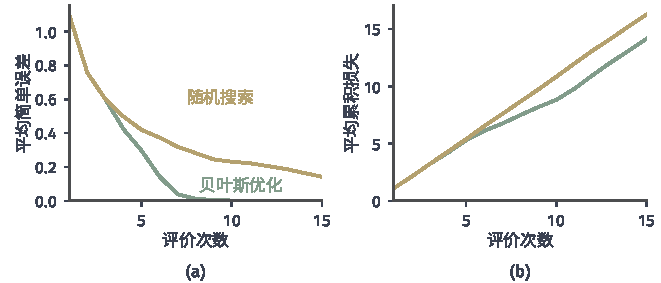
\includegraphics[width=112mm]{figures/05-optimization/05-stochastic-optimization/matplotlib/bo-regret-curves/figure.pdf}
 \caption{贯穿例上的两种误差，$200$组随机初始点的平均值。绿线是贝叶斯优化（$0.1$网格、EI），黄线是均匀随机搜索。(a)当前最好值相对$f^\star$的差；(b)累积损失~\eqref{eq:bo-cumulative-regret}。这是单个一维目标上的教学实验，不代表一般结论。}
 \label{fig:bo-regret-curves}
\end{BookInlineFigure}

\paragraph{不知道$f^\star$时}
贯穿例是人为构造的，$f^\star$可以直接算出。实际问题的最优值未知，就不能直接报告精确的推荐误差，能报告的只有依据明确的比较。可以用已知最优值的基准问题来测方法；可以用有效的下界，比如若$f$是$L$-Lipschitz的，且搜索域中每点到最近评价点的距离不超过$h$，则
\begin{equation}
 f^\star\geq\min_{i\leq T}f(\bm{x}_i)-Lh.
 \label{eq:bo-lipschitz-bound}
\end{equation}
这个不等式成立，因为最小点到某个评价点的距离不超过$h$，函数值的差不超过$Lh$。贯穿例中六个评价点的覆盖半径$h=1.5$，若取$L=2$，下界只有$-4$，松得多，可见这类下界常常只能给出保守的结论。还可以用独立的复核运行来比较候选，这能说明“比基线好多少”，不能说明“离最优多远”。

\subsection{保证的条件}
\label{sec:bo-guarantees}

贝叶斯优化有理论保证吗？可以说有，但条件比较具体。第~\ref{sec:bo-lcb}节留下的问题是：$\kappa_t$取多大，LCB才是有效的置信界？下面的定理针对有限搜索域。

\begin{theorem}[有限搜索域上的同时置信界]
\label{thm:bo-confidence}
设$\bm{C}$是有限集，$f$确实是高斯过程$F$的一个实现，读数噪声是相互独立的$N(0,\tau^2)$，$\tau\geq0$，且每个$\bm{x}_t$只依赖$\mathcal{D}_{t-1}$（可以再用与$F$独立的随机数）。对$\delta\in(0,1)$，令
\begin{equation}
 \beta_t=2\log\frac{\lvert\bm{C}\rvert\pi^2t^2}{6\delta}.
 \label{eq:bo-beta}
\end{equation}
则以至少$1-\delta$的概率，对所有$t\geq1$和所有$\bm{x}\in\bm{C}$，都有
\begin{equation}
 \lvert F(\bm{x})-m_{t-1}(\bm{x})\rvert\leq\sqrt{\beta_t}\,s_{t-1}(\bm{x}).
 \label{eq:bo-confidence}
\end{equation}
\end{theorem}

\begin{proof}
先建立高斯尾的上界。设$W\sim N(0,1)$，$c\geq0$。把积分变量写成$w=c+u$，有
\[
 \phi(c+u)=\phi(u)\,e^{-c^2/2-cu}\leq\phi(u)\,e^{-c^2/2},\qquad u\geq0.
\]
在$u\geq0$上积分，得$\mathbb{P}(W>c)\leq\frac12e^{-c^2/2}$，再由对称性，
\[
 \mathbb{P}(\lvert W\rvert>c)\leq e^{-c^2/2}.
\]

固定$t$和$\bm{x}$。给定$\mathcal{D}_{t-1}$时，$F(\bm{x})$服从$N(m_{t-1}(\bm{x}),s_{t-1}^2(\bm{x}))$。若$s_{t-1}(\bm{x})=0$，不等式~\eqref{eq:bo-confidence}必然成立；否则应用上界，
\[
 \mathbb{P}\bigl(\text{式~\eqref{eq:bo-confidence}对这一组}(t,\bm{x})\text{不成立}\mid\mathcal{D}_{t-1}\bigr)\leq e^{-\beta_t/2}.
\]
这个上界不依赖$\mathcal{D}_{t-1}$，所以对$\mathcal{D}_{t-1}$取期望后仍成立。

对所有$\bm{x}$和所有$t$作并集界。由式~\eqref{eq:bo-beta}，
\[
 e^{-\beta_t/2}=\frac{6\delta}{\lvert\bm{C}\rvert\pi^2t^2},
\]
于是失败概率不超过
\[
 \sum_{t=1}^\infty\sum_{\bm{x}\in\bm{C}}\frac{6\delta}{\lvert\bm{C}\rvert\pi^2t^2}
 =\sum_{t=1}^\infty\frac{6\delta}{\pi^2t^2}=\delta.
\]
最后一步用了$\sum_{t\geq1}1/t^2=\pi^2/6$。
\end{proof}

证明之所以能处理自适应选点，靠的是对每个$t$先以历史为条件，并对$\bm{C}$中全部点取并集，于是不管算法选哪个点，界都成立。代价是系数比单点区间大。$\lvert\bm{C}\rvert=9$，$\delta=0.1$时，
\[
 \sqrt{\beta_1}\approx3.16,\qquad\sqrt{\beta_{10}}\approx4.38,\qquad\sqrt{\beta_{100}}\approx5.33,
\]
都比单点$95\%$区间的$1.96$大得多，且随$t$缓慢增大。

有了同时置信界，LCB的单步损失立刻受控。令$\kappa_t=\sqrt{\beta_t}$，$\bm{x}_t$是$\mathrm{LCB}_{t-1}$的最小点，$\bm{x}^\star$是$f$的最小点。在式~\eqref{eq:bo-confidence}成立的事件上，
\[
 f(\bm{x}_t)\leq m_{t-1}(\bm{x}_t)+\kappa_ts_{t-1}(\bm{x}_t),
\]
而由$\bm{x}_t$的选取，
\[
 m_{t-1}(\bm{x}_t)-\kappa_ts_{t-1}(\bm{x}_t)\leq m_{t-1}(\bm{x}^\star)-\kappa_ts_{t-1}(\bm{x}^\star)\leq f^\star.
\]
两式相减，得到
\begin{equation}
 f(\bm{x}_t)-f^\star\leq2\kappa_ts_{t-1}(\bm{x}_t).
 \label{eq:bo-instant-regret}
\end{equation}
单步损失不超过所选位置的后验标准差的$2\kappa_t$倍，评价的位置不确定性越小，损失越小。

对式~\eqref{eq:bo-instant-regret}求和，再把后验标准差之和联系到\emph{最大信息增益}$\gamma_T$，就得到累积遗憾的上界：若$\tau>0$，$k(\bm{x},\bm{x})\leq1$，上述事件上对所有$T$，
\begin{equation}
 R_T\leq\sqrt{C_1T\beta_T\gamma_T},\qquad C_1=\frac{8}{\log(1+\tau^{-2})},
 \label{eq:bo-regret-bound}
\end{equation}
其中$\gamma_T$是在$T$个点上观测所能获得的最大信息增益。这一步的证明需要用到高斯信息量的链式分解和方差的求和估计，篇幅较长，读者可查阅GP-UCB方法的原始分析。对平方指数核和紧凸搜索域，$\gamma_T$随$T$只按$\log T$的多项式增长，所以$R_T/T\to0$。

这个结论的适用范围要说清楚。它要求$f$确实由所用的高斯过程产生、核和噪声方差已知、内层问题精确求解、搜索域有限；连续域需要额外的光滑性条件和离散化论证。它只对这种特定的GP置信界方法成立，不覆盖任意代理与采集函数的组合。常用的EI加上每轮重新估计超参数，就不在这个定理的范围内，模型失配和内层求解误差也都要另外检查。

表~\ref{tab:bo-claims}把几种容易混淆的说法分开。

\begin{BookInlineTable}
 \centering
 \caption{三种不同的主张。}
 \label{tab:bo-claims}
 \begin{tabular}{ll}
 \toprule
 主张&需要的条件\\
 \midrule
 单点后验可信区间&模型正确，点在观测前固定\\
 自适应的同时置信界&模型正确，并集界，系数随$t$增大\\
 有限预算找到全局最优&一般不成立，需要对$f$作额外假设\\
 \bottomrule
 \end{tabular}
\end{BookInlineTable}

最后一行值得多说一句。有限次评价只能在有限个点取值，两个点之间函数可以任意低，除非另有光滑性之类的假设，否则任何算法都不能保证找到全局最优。这也是概率模型的角色所在：它把这种假设明确写了出来，让我们知道结论依赖什么。

\section{本章小结}
\label{sec:bo-summary}

本章的出发点是预算极少的黑箱问题，$T$次评价要在有希望的区域和未知的区域之间分配。评价点负责收集信息，推荐解负责交付，选点规则只能使用已完成的观测。目标本身并不随机，概率描述的是我们对它的认识。

概率代理把已完成的观测变成对所有候选位置的预测。高斯过程用核表达“相近的位置函数值相近”，一个读数通过后验协方差影响相关的位置，后验方差只取决于评价放在哪里。超参数不确定时，直接代入估计值可能严重低估不确定性，低方差只说明在模型内不确定性小。

采集函数把预测变成分数：PI只看过线的概率，EI把幅度也计入，LCB直接按乐观值比较，Thompson采样按后验抽样选点，KG衡量一次观测对最终推荐的改善。四种规则的共同之处是都在利用与探索之间折中，不同之处在于如何折中。循环的外层是昂贵评价，内层是对采集函数的优化，而内层的求解质量也影响选点。

各种推广分别改变了循环的某一环。噪声改变了阈值的含义，需要区分潜在函数值和下一次读数，复测的价值要由信息更新的准则衡量。约束在采集分数中加入可行概率，$b_t$也改为可行读数中的最好值；要求每次试验都可行时，还需要额外的安全假设。并行使一批候选之间的相关性变得重要，未完成的试验要按预测分布平均，而不当作已有读数。成本则改变了预算的口径。

最后要分开三件事：模型给出的概率是否可信，优化的结果是否够好，计算的开销是否值得。特定的GP置信界方法有遗憾上界，但它依赖模型正确、搜索域有限和置信系数的具体取值；这些条件不满足时，算法仍可以使用，只是结论要靠实际的对照比较来支持。

